\documentclass{book}
\usepackage[spanish]{babel}

\usepackage{xunicode}
\usepackage{fontspec}
\usepackage{fullpage}

\usepackage{amsmath}
\usepackage{amssymb}
\usepackage{amscd}
\usepackage{amsthm}
\usepackage{enumerate}
\usepackage{hyperref}

\usepackage{tikz}
\usetikzlibrary{babel}

\begin{document}

\title{Matemáticas II}
\author{
\includegraphics{../../logos/128x128-mexico.png}}

\maketitle

\tableofcontents

\section*{Introducción}

Este libro está basado sobre el programa del subsecretaría de educación media
superior en México y cobre la parte ``Matemática I''.
Fue realizado para el proyecto BELLA
(Biblioteca Electrónica de Libros Libres para el Aprendizaje) cuyo el objetivo
es crear libros electrónicos bajo una licencia libre y usando
tecnologías Web.

Este libro está distribuido como una Firefox OS aplicación Web que puede ser leída en Firefox OS dispositivos y otros sistemas compatibles como Android.
Puede encontrar más libros del proyecto BELLA, interactiva
ejercicios, exámenes o otras Web apps sobre el Firefox MarketPlace. Aquí están
algunas aplicaciones del proyecto BELLA recomendadas para la parte
``Matemática I'':

\begin{itemize}
\item Divipoli (capítulo 5)
\item Sislineal (capítulos 7 y 8)
\item Cuadratica (capítulo 9)
\end{itemize}

Mozilla es una comunidad de tecnólogos, pensadores y desarrolladores que
trabajan para que Internet siga vivo y accesible, para que todos seamos
colaboradores informados y creadores de la Web. Si quiere participar, contacte
la comunidad de Mozilla México o del proyecto MathML de Mozilla.

\section*{Derecho de autor}

Este libro está bajo la
licencia Creative Common License BY-SA 4.0. Usted es libre de:

\begin{enumerate}
\item Compartir — copiar y redistribuir el material en cualquier medio o formato
\item Adaptar — remezclar, transformar y crear a partir del material 
\end{enumerate}

Bajo las condiciones siguientes:

\begin{enumerate}
\item Reconocimiento — You must give appropriate credit, provide a link to the license, and indicate if changes were made. You may do so in any reasonable manner, but not in any way that suggests the licensor endorses you or your use. 
\item CompartirIgual — Si remezcla, transforma o crea a partir del material, deberá difundir sus contribuciones bajo la misma licencia que el original. 
\end{enumerate}

No hay restricciones adicionales — No puede aplicar términos legales o medidas tecnológicas que legalmente restrinjan realizar aquello que la licencia permite.

\chapter{Utilizas triángulos: ángulos y relaciones métricas}

\section{Tipo de ángulos y relaciones entre ángulos}

Un ángulo es la parte del plano entre dos semirrectas con el mismo punto de
origen. La medida de este ángulo se llama amplitud. Un grado (sexagesimal)
es la amplitud de un ángulo igual a $\frac{1}{360}$ de la circunferencia.
Si los semirrectas no son coincidentes o alineadas, determinan dos ángulos, uno
convexo (el de menor amplitud) y otro cóncavo (el de mayor amplitud).

\begin{center}
\begin{tabular}{| c | c  | c |}
\hline
Tipo & Amplitud & \\
\hline
Ángulo nulo & $A = 0°$ & 
\begin{tikzpicture}
   \draw (0,0) -- (1,0);
 \end{tikzpicture} \\
\hline
Ángulo agudo & $0° < A < 90°$ &
 \begin{tikzpicture}
   \draw (1,0) -- (0,0) -- (0.707,0.707);
   \draw (.5,0) arc (0:45:.5)[color=red];
 \end{tikzpicture} \\
\hline
Ángulo recto & $A = 90°$ &
 \begin{tikzpicture}
   \draw (1,0) -- (0,0) -- (0,1);
   \draw (.2,0) -- (.2,.2) -- (0,.2)[color=red];
 \end{tikzpicture} \\
\hline
Ángulo obtuso & $90° < A < 180°$ &
 \begin{tikzpicture}
   \draw (1,0) -- (0,0) -- (-0.707,0.707);
   \draw (.5,0) arc (0:135:.5)[color=red];
 \end{tikzpicture} \\
\hline
Ángulo llano & $A = 180°$ & 
\begin{tikzpicture}
   \draw (1,0) -- (0,0) -- (-1,0);
   \draw (.5,0) arc (0:180:.5)[color=red];
 \end{tikzpicture}\\
\hline
Ángulo oblicuo & $A \neq 0°, 90°, 180°, 270°, 360°$ &\\
\hline
Ángulo completo o perigonal & $A = 360°$&
\begin{tikzpicture}
   \draw (0,0) -- (1,0);
   \draw (.5,0) arc (0:360:.5)[color=red];
 \end{tikzpicture} \\
\hline
\end{tabular}
\end{center}

\subsection{Ejercicio 1}

Indique el tipo de los ángulos de medidas siguientes:
35°, 180°, 45°, 200°, 90°, 350°, 0°, 100°.

\subsection{Definición}

Dos ángulos son complementarios si sus medidas suman 90°:

\begin{center}
 \begin{tikzpicture}
   \draw (0,0) -- (2,0);
   \draw (0,0) -- (1.7320,1);
   \draw (0,0) -- (0,2);
   \draw (0,.2) -- (.2,.2) -- (.2,0);
   \draw (.5,0) arc (0:30:.5)[color=red] node(A){};
   \draw (A) arc (30:90:.5)[color=blue];
 \end{tikzpicture}

\end{center}

Dos ángulos son suplementarios si sus medidas suman 180°:

\begin{center}
 \begin{tikzpicture}
   \draw (0,0) -- (2,0);
   \draw (0,0) -- (1.7320,1);
   \draw (0,0) -- (-2,0);
   \draw (.5,0) arc (0:30:.5)[color=red] node(A){};
   \draw (A) arc (30:180:.5)[color=blue];
 \end{tikzpicture}
\end{center}

En la figura siguiente, los ángulos rojos son dichos opuestos por el vértice.
Son suplementarios del ángulo azul y entonces iguales:

\begin{center}
 \begin{tikzpicture}
   \draw (-1.5,0) -- (1.5,0);
   \draw (-1,-1) -- (1,1);
   \draw (1,0) arc (0:45:1)[color=red] node(A){};
   \draw (A) arc (45:180:1)[color=blue];
   \draw (-1,0) arc (180:225:1)[color=red];
 \end{tikzpicture}

\end{center}


Consideramos dos rectas paralelas y una transversal a ellas. En la figura
siguiente, los ángulos de mismos colores son dichos correspondientes y tienen
la misma amplitud:

\begin{center}

 \begin{tikzpicture}
   \draw (0,0) -- (5,0);
   \draw (0,1) -- (5,1);
   \draw (1,-1) -- (4,2);
   \draw (3.5,1) arc (0:45:.5)[color=red] node(A){};
   \draw (A) arc (45:180:.5)[color=blue] node(B){};
   \draw (B) arc (180:225:.5)[color=orange] node(C){};
   \draw (C) arc (225:360:.5)[color=green];

   \draw (2.5,0) arc (0:45:.5)[color=red] node(AA){};
   \draw (AA) arc (45:180:.5)[color=blue] node(BB){};
   \draw (BB) arc (180:225:.5)[color=orange] node(CC){};
   \draw (CC) arc (225:360:.5)[color=green];

 \end{tikzpicture}

\end{center}

En la figura siguiente, los ángulos de mismos colores son dichos
alternos y tienen la misma amplitud:

\begin{center}

 \begin{tikzpicture}
   \draw (0,0) -- (5,0);
   \draw (0,1) -- (5,1);
   \draw (1,-1) -- (4,2);
   \draw (3.5,1) arc (0:45:.5)[color=red] node(A){};
   \draw (A) arc (45:180:.5)[color=blue] node(B){};
   \draw (B) arc (180:225:.5)[color=orange] node(C){};
   \draw (C) arc (225:360:.5)[color=green];

   \draw (2.5,0) arc (0:45:.5)[color=orange] node(AA){};
   \draw (AA) arc (45:180:.5)[color=green] node(BB){};
   \draw (BB) arc (180:225:.5)[color=red] node(CC){};
   \draw (CC) arc (225:360:.5)[color=blue];

 \end{tikzpicture}

\end{center}

\subsection{Ejercicio 2}

Determine si los ángulos de amplitudes siguientes son complementarios,
suplementarios ningún de los dos:

\begin{itemize}
  \item ¿20° y 160°?
  \item ¿35° y 65°?
  \item ¿28° y 62°?
  \item ¿83° y 97°?
  \item ¿18° y 172°?
\end{itemize}

\subsection{Ejercicio 3}

Indique el ángulo complementario y suplementario de los ángulos siguientes de
amplitudes siguientes: 20°, 57°, 88°, 0°, 90°.

\subsection{Ejercicio 4}

Consideramos dos rectas paralelas y una transversal a ellas.
Indique los ángulos que son correspondiente y alternos con el ángulo rojo.
¿Si la amplitud del ángulo azul es 145°, cuales son las amplitudes de los otros?

\begin{center}

 \begin{tikzpicture}
   \draw (0,0) -- (8,0);
   \draw (0,2) -- (8,2);
   \draw (1,-1) -- (7,3);

   \draw (6.5,2) arc (0:35:1)[color=red] node(A){};
   \draw (A) arc (35:180:1)[color=blue] node(B){};
   \draw (B) arc (180:215:1)[color=green];

   \draw (3.5,0) arc (0:35:1)[color=purple];
   \draw (1.5,0) arc (180:215:1)[color=orange];

 \end{tikzpicture}

\end{center}

\section{Triángulos, lados y ángulos}

Podemos definir un (único) triángulo a partir de las medidas de sus lados
$a, b, c$ si y sólo si $c$ es el $a < b + c$, $b < a + c$ y $c < a + b$.

\begin{center}

 \begin{tikzpicture}
   \path (0,0) edge node[above]{$a > b + c$} (5,0) ;
   \path (0,0) edge node[above]{$b$} (2,1) ;
   \path (5,0) edge node[above]{$c$} (4,.5) ;
 \end{tikzpicture}

\end{center}

Un triángulo es escaleno, si todos sus lados tienen longitudes diferentes.
Un triángulo es isósceles si tiene dos lados iguales. Un triángulo equilátero
tiene sus tres lados iguales.

Podemos definir un triángulo a partir de las medidas de dos ángulas
$\alpha, \beta > 0$ si y sólo si $\alpha + \beta < 180°$. Obtenemos una
infinidad de triángulos con los mismos amplitudes si hacemos variar
proporcionalmente las longitudes de los lados. Si $\gamma$ es la
medida del tercer ángulo, tenemos
%%
$$
\alpha + \beta + \gamma = 180°
$$

Un triángulo es escaleno, si y solo si todos sus ángulos tienen amplitudes
diferentes.
Un triángulo es isósceles, si y solo si tiene dos ángulos de misma amplitud.
Es equilátero si y solo si tiene sus tres ángulos de misma amplitud, es decir
$\frac{180}{3} = 60°$.

Si una de los ángulo es recto (90°), el triángulo es dicho rectángulo. En
en otro caso es dicho oblicuángulo.

\begin{center}
 \begin{tikzpicture}
   \draw (0,0) -- (3,0) -- (3,4) -- (0,0);
   \draw (2.8,0) -- (2.8,.2) -- (3,.2);
 \end{tikzpicture}
\end{center}

Un triángulo es obtusángulo si uno de sus ángulos es obtuso (mayor de 90°) y
acutángulo si todos son agudos (menor de 90°).

\subsection*{Ejercicio 5}

Cuando es posible, dibuje un triángulo con las condiciones siguientes y indique
el tipo del triángulo.

\begin{itemize}
\item Triángulo de lados 3, 7, 3.
\item Triángulo de lados 3, 5, 3.
\item Triángulo de lados 3, 3, 3.
\item Triángulo de ángulos 90°, 75° y 25°.
\item Triángulo con dos lados de lado 7 formando un ángulo recto.
\item Triángulo de lados 6, 8, 10.
\item Triángulo con dos ángulos de medida 60°.
\item Triángulo con dos ángulos de medida 70° y 40°.
\item Triángulo de lados 7, 3, 10.
\item Triángulo con dos ángulos de medida 50° y 10°.
\item Triángulo con dos ángulos complementarios de medida diferentes de 45°.
\item Triángulo de lados 7, 8, 9.
\end{itemize}

\subsection{Ejercicio 6 (Tales)}

Consideramos un círculo de diámetro $[AB]$ y centro $O$. Sea $C$ otro punto
($\neq A,B$) sobre el círculo. ¿Cual es el tipo de los triángulos $OBC$ y
$OAC$? Si $\alpha = \widehat{BAC}$ y $\beta = \widehat{ABC}$ exprese el
ángulo $\widehat{BCA}$ en función de $\alpha, \beta$. Exprese la
suma de los ángulos del triángulo $ABC$ en función de $\alpha, \beta$. Deducir
que $ABC$ es rectángulo en $C$.

\section{Soluciones de los ejercicios}

\subsection*{Ejercicio 1}

agudo y oblicuo, llano, agudo y oblicuo, oblicuo, recto, oblicuo, nulo, obtuso y
oblicuo.

\subsection*{Ejercicio 2}

\begin{itemize}
  \item suplementario
  \item ningún de los dos
  \item complementario
  \item suplementario
  \item ningún de los dos
\end{itemize}

\subsection*{Ejercicio 3}

Las medidas de los ángulos complementarios son 70°, 33°, 2°, 90°, 0°.
Las medidas de los ángulos suplementarios son 160°, 123°, 92°, 90°, 180°.

\subsection*{Ejercicio 4}

El ángulo naranja es alterno con el ángulo rojo, el ángulo ṕurpuro es
correspondiente con el ángulo rojo. Los ángulos rojo y verde son opuestos
por el vértice y entonces iguales. Por la primera pregunta,
es también la medida de los ángulos naranja y ṕurpuro.

\subsection*{Ejercicio 5}

\begin{itemize}
\item No es posible por que $7 > 3 + 3$.
\item obtusángulo, isósceles, oblicuángulo.
\item acutángulo, equilatero, oblicuángulo.
\item No es posible por que $90 + 75 + 25 \neq 180$.
\item escaleno, rectángulo.
\item acutángulo, equilatero, oblicuángulo.
\item acutángulo, isósceles, oblicuángulo.
\item No es posible por que $10 = 3 + 7$.
\item obtusángulo, escaleno, oblicuángulo.
\item escaleno, rectángulo.
\item acutángulo, escaleno, oblicuángulo.
\end{itemize}

\subsection{Ejercicio 6 (Tales)}

$OBC$ y $OAC$ son isósceles por que $OA = OB = OC$ es el radio del círculo.
Entonces $\widehat{OAC} = \widehat{OCA} = \alpha$ y
$\widehat{OBC} = \widehat{OCB} = \beta$.

Tenemos $\widehat{BCA} = \alpha+\beta$ y
la suma de de los ángulos de $ABC$ es
$180° = \widehat{ABC} + \widehat{BCA} + \widehat{CAB} =
\beta + {(\alpha+\beta)} + \alpha = 2\left(\alpha+\beta\right)$.

Finalmente, $\widehat{BCA} = 90°$ y $ABC$ es rectángulo en $C$.

\chapter{Utilizas magnitudes y números reales}

\section{Números reales}

\subsection*{Resumen}

Los números reales (designados por $\mathbb R$) pueden ser representatos como
puntos sobre una recta.

\begin{center}
\begin{tikzpicture}
  \draw (-3,0) --(3,0);
  \path (-4,0) node (minf) {$\ldots$};
  \path (4,0) node (inf) {$\ldots$};
  \draw (-1,-.1) --(-1,.1);
  \draw (-2,-.1) --(-2,.1);
  \draw (0,-.1) --(0,.1);
  \draw (1,-.1) --(1,.1);
  \draw (2,-.1) --(2,.1);
  \path (0,.5) node (n0) {$0$};
  \path (1,.5) node (n1) {$1$};
  \path (2,.5) node (n2) {$2$};
  \path (-1,.5) node (nm1) {$-1$};
  \path (-2,.5) node (nm2) {$-2$};
\end{tikzpicture}
\end{center}

Los números naturales (designados por $\mathbb N$) son $0, 1, 2, 3, \ldots$. Si
además incluyemos los números negativos, obtenemos los números enteros
(designados por $\mathbb Z$: $\ldots -3, -2, -1, 0, 1, 2, 3, \ldots$).
Los números de la forma
$\frac{p}{q}$ donde $p \in \mathbb Z$ y $q \in \mathbb N \setminus \{0\}$ se
llaman los racionales (designados por $\mathbb Q$). En particular si considemos
los racionales donde $q=10^n$ para algun $n \in \mathbb N$, obtenemos los
número decimales como $-494.1627$.
Los reales que no son racionales se llaman números irracionales.

\begin{center}
\begin{tikzpicture}
  \draw (0,0) rectangle(7,7);
  \path (3,0.5) node (R) {$\mathbb R$ Números reales $\sqrt{2}, \pi$};
  \draw (.5,1) rectangle(6.5,6.5);
  \path (4,1.5) node (Q) {$\mathbb Q$: $-\frac{8}{7}, \frac{2}{3}$};
  \draw (1,2) rectangle(6,6);
  \path (4,2.5) node (D) {Números decimales $-2.5$};
  \draw (2,3) rectangle(5.5,5.5);
  \path (3,3.5) node (Z) {$\mathbb Z$: $-7$};
  \draw (3,4) rectangle(5,5);
  \path (4,4.5) node (N) {$\mathbb N$: $0, 6$};
\end{tikzpicture}
\end{center}

\subsection*{Ejemplos}

\begin{enumerate}
\item $364$ es un número natural.
\item $-36$ es un número entero (negativo) pero no es un número natural.
\item $0.8$ es un número decimal pero no es entero.
\item $\frac{1}{3}$ es un numero racional pero no es un número decimal.
\item $\sqrt{2}$ es un numero real pero no es un número racional (ejercicio 2).
\end{enumerate}

\subsection*{Ejercicio 1}

Calcular $3n$ y $3{(n+1)}$ para $n = 3, 33, 333, 3333, \ldots$ etc y $10^m$ para
$m = 0, 1, 2, 3, \ldots$.

Suponemos que $\frac{1}{3}$ se puede escribir como un decimal
$\frac{n}{10^m}$ donde $n \in \mathbb N$ y $m \in \mathbb N$. ¿Es eso posible?

\subsection*{Ejercicio 2}

Clasifiar los ńumeros reales siguientes (enteros, racionales...)

\begin{enumerate}
\item $6$
\item $-2$
\item $2.5$
\item $-7.0$
\item $\frac{3}{2}$
\item $-\frac{1}{3}$
\item $\frac{16}{8}$
\item $\sqrt{2}$
\item $\sqrt{49}$
\item $\sqrt{\frac{16}{25}}$
\item $\sqrt[3]{0.125}$
\end{enumerate}

\subsection*{Ejercicio 3 (difícil antes del capítulo IV)}

Si $n$ es un entero, verifia que ${(2n+1)}^2 = 2{(2n^2+2n)} + 1$ y que
${2n}^2 = 2{(2n)}$. Cuál es la relación entre la paridad de un entero y
de su cuadrado?

Consideramos $p \in \mathbb Z$ y $q \in {\mathbb N} \setminus \{0\}$
tal que $\sqrt{2} = \frac{p}{q}$ y $q$ el más pequeño posible.
Muestrar que $p^2$ es un número par y entonces $p$ también.

Si escribimos $p = 2n$, muestrar que $q^2 = 2n^2$ y entonces $q$ es par.
Encuentra $p'$ y $q'$ tal que $q' < q$ y $\sqrt{2} = \frac{p'}{q'}$,
contradiciendo la hipótesis original.

\subsection*{Ejercicio 4}

Ubica en la recta numérica de números reales los números siguientes: $0, 1, 8,
0.25, -4, \frac{9}{4}, \frac{10}{3}, -\sqrt{2}$.

\subsection*{Ejercicio 5 (introducción informal a los números complejos)}

Suponemos que existe un número $i$ tal que $i^2 = -1$ y consideramos el
conjunto de los complejos
$\mathbb{C} = \left\{ a + ib, a \in \mathbb{R}, b \in \mathbb{R} \right\}$.
Si $z = a + ib$, $a$ es parte real y $b$ la parte imaginaria. Si $a = 0$,
$z$ es dicho número imaginario puro.
El conjugado de $z$ es $\bar{z} = a - i b$ y el módulo de $z$ es
${|z|} = \sqrt{a^2 + b^2}$. El complejo $z \neq 0$
puede ser representado en un plano de la manera siguiente:

\begin{center}
\begin{tikzpicture}
  \draw (0,0) node[left] {$0$} circle (2);
  \draw[style=dashed,color=gray] (0,0) circle (3);
  \draw[color=red] (0,0) -- (0.75,1.299038105676657) node[left] {$\rho$} --(1.5,2.598076211353315) node[right] {$z=a+ib$};
  \draw[->] (0,0) -- (4,0);
  \draw[->] (0,0) -- (0,4);
  \path (2,0) node[right] {$1$};
  \path (0,2) node[above] {$i$};
  \draw[style=dashed,color=blue] (1.5,2.598076211353315) -- (1.5,0) node[right] {$a$};
  \draw[style=dashed,color=blue] (1.5,2.598076211353315) -- (0,2.598076211353315) node[above] {$b$};
  \draw[color=green] (.5,0) arc (0:60:.5) node[right] {$\varphi$};
\end{tikzpicture}
\end{center}

\begin{enumerate}
\item ¿Cómo definir la suma, resta, producto de números complejos?
\item  $z \bar{z}$ y deducir un número $z'$ tal que $z z' = 1$. ¿Como definir
  el inverso de un número complejo y la división de dos complejos?
\item Muestrar que para cada número real $r \neq 0$, hay dos complejos
  $z_1 \neq z_2$ tal que $z_1^2 = z_2^2 = r$. ¿Que decir de esos números segun
  el signo de $r$?
\item En la representación gráfica, $\rho$ es el módulo de $z$ y el angulo
  $\varphi$ es llamado el argumento. Expresar $a, b$
  en función de $\rho$ y $\varphi$.
\item Cómo interpretar gráficamente la suma, resta y conjugación de complejos?
\item Recordar las formulas para el coseno y seno de la suma de dos ángulos.
  Si $z_1, z_2$ tienen módulos y argumentos $\rho_1, \varphi_1$ y
  $\rho_2, \varphi_2$, ¿Cómo se expresa el producto $z_1 \times z_2$ en función
  de esos parametros? ¿Cómo interpretar gráficamente el producto de dos
  complejos?
\item Deducir que para cada número real $r \neq 0$ sólo hay dos $z$ tal
  que $z^2 = r$ . ¿Que decir de $r=0$?
\end{enumerate}

\section{Operaciones}

\subsection*{Resumen}

Las operaciones vistas para los números positivos existen también para
los reales:

\begin{enumerate}
\item Suma: si $p, q$ son números positivos, tenemos
  $p + -q = p - q$, $-p + q = q - p$ y $-p + -q = -{(p+q)}$.
\item Resta: si $p, q$ son números positivos, tenemos
  $p - -q = p + q$, $-p - q = -{(p + q)}$ y $-p - -q = q - p = -{(p - q)}$.
\item Multiplicación: si $p, q$ son números positivos, tenemos
  $p \times -q = -p \times q = -{(p \times q)}$ y
  $-p \times -q = p \times q$
\item División: $p, q$ son números positivos y $q \neq 0$, tenemos
  $p / -q = -p / q = -{(p / q)}$ y
  $-p / -q = p / q$
\item $p^{-n} = \frac{1}{p^n}$ para $p$ real y $n$ entero.
\item Si $p$ es un número positivo y $n$ es entero,
  ${-p}^{n} = p^n$ si $n$ es par y ${-p}^{n} = -p^n$ si $n$ es impar.
\item $\sqrt[n]{-p} = -\sqrt[n]{p}$ si $n$ es impar y $p$ positivo. No podemos
  definir un tal número real si $n$ es par y $p > 0$.
\end{enumerate}

\subsection*{Ejemplos}

\begin{enumerate}
\item $-1 + -5 = -6$, $5 - 7 = -2$
\item $5 - -6 = 11$, $-7 - 8 = -15$
\item $-2 \times 3 = -6$, $-2 \times -3 = 6$
\item $-8 / 4 = -2$, $-10 / -5 = 2$
\item $2^-3 = \frac{1}{2^3} = \frac{1}{8} = 0.125$, ${(-2)}^{3} = -8$
\item $\sqrt[3]{-27} = -3$
\end{enumerate}

\subsection*{Ejercicio 6}

Calcular:

\begin{enumerate}
\item ${(-1 + 6)} \times {(-2)}^3$
\item $\frac{-5 + -2}{7} + 2$
\item $2 \sqrt[3]{(10 - 11 \times 4 + 14 / 2)}$
\item $8 - \left(\frac{2}{-3}\right)^{-2} + 1$
\end{enumerate}

\subsection*{Ejercicio 7}

El kelvin es la unidad de temperatura del Sistema Internacional de Unidades.

Otras unidades usadas par medir la temperatura son los grados Fahrenheit y
Celcius. Para convertir una tempentura $T$ en kelvin a una tempentura en grado
Fahrenheit, hay que multiplicar $T$ por $\frac{9}{5}$ y restar $459.67$.
Para convertir una tempentura $T$ en grado Celcius a una tempentura $T$ en
kelvin, hay que añadir $273.15$.

Si la temperatura era $59°F$ por la mañana y ha crecido de $5\%$. ¿Cuál es ahora
la temperatura en grado Celcius?

\section{Razones, tasas, proporciones y variaciónes}

\subsection*{Resumen}

Una razón es fracción que compara dos cantidades. Por ejemplo,
tres de cada diez mujeres:
$\frac{3}{10}$, $3:10$, $3$ de $10$. Una tasa es una razón de dos cantidades
diferentes. $100$ kilometros por $2$ horas: $\frac{100}{2}$, $100 : 2$,
$100$ de $2$.

Una proporción es dos razones o fracciones iguales $\frac{a}{b} = \frac{c}{d}$.
$a$ es a $c$ como $b$ es a $d$. Los extremos de la proporción son $a$ y $d$,
mientras $b$ y $c$ son llamados los medios. El producto de los medios es igual
al producto de los extremos: $a d = c b$.

Una variación es la evolución de una variable ```a'' con respecto a otra
``b'', por una razón ``k''. Una variacíon es directa si la primera variable
aumenta cuando la otra aumenta ($a = k \times b$) y inversa si la
primera variable disminuye cuando la otra aumenta ($a = k / b$).

\subsection*{Ejercicio 8}

\begin{enumerate}
\item En una tienda, 1.5kg de tomate cuesta 24MXN. En otra tienda, 300g de
  tomate cuesta 5MXN. ¿Cuál es la mejor compra?
\item Dos botellas de agua cuestan 16.72MXN. ¿Cuantos botellas podemos comprar
  con 50.16MXN?
\item En electricidad, la ley de Ohm relaciona el voltaje $V$, con la carga
  $R$, y la corriente $I$ con la relación $V=RI$. Indicata el tipo de
  variación de $R$ con respecto a $I$.
\end{enumerate}

\section{Soluciones de los ejercicios}

\subsection*{Ejercicio 1}

Obtenemos $9, 99, 9999, 99999$, $12, 102, 1002, 10002$ y
$1, 10, 100, 1000, 10000, \ldots$. Nos damos cuenta de que $10^m$ nunca es divisible
por $3$. Entonces $\frac{1}{3} = \frac{n}{10^m}$ no es posible o tendríamos
$10^m = 3n$.

\subsection*{Ejercicio 2}

\begin{enumerate}
\item $6$ es un número natural.
\item $-2$ es un número entero pero no es natural.
\item $2.5 = \frac{25}{10^1}$ es un número decimal pero no es entero.
\item $-7.0 = -7$ es un número entero pero no es natural.
\item $\frac{3}{2} = 1.5$ es un número decimal pero no es entero.
\item $-\frac{1}{3}$ es un numero racional pero no es decimal por ejercicio 1.
\item $\frac{16}{8} = 2$ es un número natural.
\item $\sqrt{2}$ es un numero real pero no es racional por ejercicio 3.
\item $\sqrt{49} = 7$ es un número natural.
\item $\sqrt{\frac{16}{25}} = \frac{4}{5} = \frac{8}{10^1} = 0.8$ es un número
decimal pero no es entero.
\item $\sqrt[3]{0.125} = 0.5$ es un número decimal pero no es entero.
\end{enumerate}

\subsection*{Ejercicio 3}

${(2n+1)}^2 = {(2n+1)}{(2n+1)} = 4n^2 + 2n + 2n + 1 = 4n^2 + 4n + 1 =
2{(2n^2+2n)} + 1$ y ${2n}^2 = 4n^2 = 2{(2n)}$. Entonces
un entero $N$ es par si y solo si $N^2$ es par.

Si $\sqrt{2} = \frac{p}{q}$, $2 = \frac{p^2}{q^2}$ y entonces
$p^2 = 2q^2$ es par. Por el primer párafo, $p$ es par y se puede escribir
$p = 2n$ para alguno entero $n$.

Ahora, tenemos $2q^2 = {(2n)}^2 = 4n^2$ y entonces $q^2 = 2n^2$ es par.
Aún podemos escribir $q = 2m$ para alguno entero $n$ y finalmente
$\sqrt{2} = \frac{2n}{2m} = \frac{n}{m}$. Si ponemos $p' = n$ y $q' = m$
encontramos una contradición.

\subsection*{Ejercicio 4}

$0.25 = \frac{1}{4}$, $\frac{9}{4} = 2 + \frac{1}{4}$,
$\frac{10}{3} = 3 + \frac{1}{3}$, $-\sqrt{2} \approx -1.414213562373095$

\begin{center}
\begin{tikzpicture}
  \draw (-9,0) --(9,0);
  \draw (1,-.2) --(1,.2);
  \draw (2,-.1) --(2,.1);
  \draw (3,-.1) --(3,.1);
  \draw (4,-.1) --(4,.1);
  \draw (5,-.1) --(5,.1);
  \draw (6,-.1) --(6,.1);
  \draw (7,-.1) --(7,.1);
  \draw (8,-.1) --(8,.1);
  \draw (0,-.2) --(0,.2);
  \draw (-1,-.1) --(-1,.1);
  \draw (-2,-.1) --(-2,.1);
  \draw (-3,-.1) --(-3,.1);
  \draw (-4,-.1) --(-4,.1);
  \draw (-5,-.1) --(-5,.1);
  \draw (-6,-.1) --(-6,.1);
  \draw (-7,-.1) --(-7,.1);
  \draw (-8,-.1) --(-8,.1);
  \path (0,.5) node (n0) {$0$};
  \path (1,.5) node (n1) {$1$};
  \path (2,.5) node (n2) {$2$};
  \path (3,.5) node (n3) {$3$};
  \path (4,.5) node (n4) {$4$};
  \path (-4,.5) node (nm4) {$-4$};

  \draw (0.25,-.1) --(0.25,2);
  \draw (0.5,-.1) --(0.5,.1);
  \draw (0.75,-.1) --(0.75,.1);
  \path (0.25,2.2) node (n025) {$0.25$};

  \draw (2.25,-.1) --(2.25,2);
  \path (2.25,2.2) node (n94) {$\frac{9}{4}$};

  \draw (3.333333333333,-.1) --(3.333333333333,2);
  \draw (3.666666666666,-.1) --(3.666666666666,.1);
  \path (3.333333333333,2.2) node (n103) {$\frac{10}{3}$};

  \draw (-1.414213562373095,-.1) --(-1.414213562373095,2);
  \path (-1.414213562373095,2.2) node (nmsqrt2) {$-\sqrt{2}$};


\end{tikzpicture}
\end{center}

\subsection*{Ejercicio 5 (introducción informal a los números complejos)}

\begin{enumerate}
\item Sean $z = a+ib$ y $z' = a'+ib'$.
  $z + z' = {(a+a')} + i (b+b')$, $z - z' = {(a-a')} + i {(b-b')}$.
  $z \times z' = {a a'} + {i ab'} + {i a'b} + {(ib)(ib')} =
  {(aa' - bb')} + i {(ab' + a'b)}$
\item $z \bar{z} = a^2 + b^2 + i {(ab - ab)} = {|z|}^2$
  Entonces si $z' = \frac{\bar{z}}{{|z|}^2}$, $z z' = 1$. Definimos el inverso
  de $z$ por $z^{-1} = \frac{\bar{z}}{{|z|}^2}$ y
  $\frac{z_1}{z_2} = z_1 z_2^{-1}$.
\item Si $r > 0$ ya sabemos que $z_1 = -\sqrt{r}$ y $z_2 = \sqrt{r}$ convienen.
  Si $r < 0$, notamos que $z_1 = -i\sqrt{r}$ y $z_2 = i\sqrt{r}$ convienen
  tambíen porque $i^2 = -1$. Si $r > 0$ $z_1,z_2$ son reales y si $r < 0$,
  esos son imaginario puro.
\item $a = \rho {\cos(\varphi)}$, $b = \rho {\sin(\varphi)}$
\item La suma y resta se intepretan como suma y resta de vectores. La conjucación como la simetria en el eje $X$.
\item $z_1 z_2 = {\rho_1 \rho_2} \left({\cos(\varphi_1 + \varphi_2)} + i
  {\sin(\varphi_1 + \varphi_2)} \right)$. Entonces el módulo del producto es el
  producto de los modulos y el argumento del producto es la suma de los argumentos.
\item Si $z^2 = r$ y tenemos ${|z|}^2 = {|r|}$ y $2 \varphi \equiv 0 \mod 360°$ ($r > 0$) o $2 \varphi \equiv 180 \mod 360°$ ($r < 0$).
  Entonces $|z| = \sqrt{|r|}$ y $\varphi \equiv 0, 180 \mod 360°$ ($r > 0$)
  o $\varphi \equiv 90, 270 \mod 360°$ ($r < 0$), y esos son los soluciones
  encontradas arriba. Si $z \neq 0$, ${|z|} \neq 0$ y ${|z^2|} =
  {|z|}^2 \neq 0$. Entonces el único complejo tal que $z^2 = 0$ es $z = 0$.
\end{enumerate}

\subsection*{Ejercicio 6}

\begin{enumerate}
\item $-40$
\item $1$
\item $-6$
\item $\frac{27}{4}$
\end{enumerate}

\subsection*{Ejercicio 7}

Hay que trabajar con la temperatura absoluta (en kelvin)!

$59°F$ corresponde a ${(59+459.67)} \times \frac{5}{9} = 288.15$ kelvin.
Si ha crecido de $5\%$, ahora la temperatura es
$288.15 \times \left(1+\frac{5}{100}\right)= 302.5575$ kelvin, es decir
$302.5575 - 273.15 \approx 29°C$

\subsection*{Ejercicio 8}

\begin{enumerate}
\item $\frac{24}{1.5} = \frac{48}{3}$ mientras
  $\frac{5}{.3} = \frac{50}{3}$. Entonces la primera es la mejor.
\item Si $n$ es el número de agua, tenemos
  $\frac{16.72}{2} = \frac{50.16}{n}$ entonces
  $n = \frac{2 \times 50.16}{16.72} = 6$ botellas.
\item Tenemos $R = \frac{V}{I}$ entonces es una variación inversa de razón $V$.
\end{enumerate}

\chapter{Resuelves problemas de semejanza de triángulos y teorema de pitágoras}

\section{Triángulos semejantes}

\subsection{Definición}

Dos triángulos $ABC$ y $DEF$ son semejantes si tiene una de las propiedades
equivalentes:

\begin{itemize}
\item $\widehat{A} = \widehat{D}, \widehat{B} = \widehat{E},
  \widehat{C} = \widehat{F}$
\item $\frac{DE}{AB} = \frac{EF}{BC} = \frac{FD}{CA}$
\end{itemize}

\subsection{Ejercicio 1}

Encontre dos triángulos semejantes que no son congruentes.
¿Es la recíproca posible?

\subsection{Ejercicio 2}

Sean dos triángulos $ABC$ y $DEF$.

\begin{enumerate}
\item Mostrar que
  si $\widehat{A} = \widehat{D}, \widehat{B} = \widehat{E}$, son semejantes.
\item ¿Que decir si sólo tenemos $\widehat{A} = \widehat{D}$?
\item ¿Y si sólo tenemos $\frac{DE}{AB} = \frac{EF}{BC}$?
\end{enumerate}

\subsection{Teorema de Tales}

Si en un triángulo se traza una línea paralela a cualquiera de sus lados, se
obtiene un triángulo que es semejante al triángulo dado.

Por ejemplo, en la figura siguiente, consideramos un triángulo $ABC$ y trazamos
3 rectas (roja, verde y azul) paralela al lado $AB$. Obtenemos tres
triángulos ${A_1B_1C_1}, {A_2B_2C_2}, {A_3B_3C_3}$ semejantes a $ABC$:

\begin{center}
 \begin{tikzpicture}
   \draw (0,0)node[below left] {$A$} -- (0,4) node[above left] {$B$}
   -- (3,1) node[right] {$C$} -- (0,0)[color=orange];
   \draw (6,-2) -- (3,1) -- (6,2)[dashed];
   \draw (0,0) -- (-3,-1)[dashed];
   \draw (0,4) -- (-3,7)[dashed];

   \draw (-1,7) -- (-1,5)node[above left] {$B_1$} --
   (-1,-0.33333333333333)node[below left] {$A_1$} -- (-1,-3)[red];
   \draw (2,7) -- (2,2)node[above right] {$B_2$} --
   (2,0.66666666666666)node[below right] {$A_2$} -- (2,-3)[green];
   \draw (5,7) -- (5,1.66666666666666)node[above right] {$A_3$}
   -- (5,-1)node[below right] {$B_3$} -- (5,-3)[blue];
   \
 \end{tikzpicture}
\end{center}

y tenemos:

$$
\frac{CA}{CA_1} = \frac{CB}{CB_1} = \frac{AB}{A_1B_1}
$$
%%
$$
\frac{CA_2}{CA} = \frac{CB_2}{CB} = \frac{A_2B_2}{AB}
$$
%%
$$
\frac{CA}{CA_3} = \frac{CB}{CB_3} = \frac{AB}{A_3B_3}
$$

\subsection{Ejercicio 3 (Tales)}

En la figura precedente, utilice los resúltados del cápitulo uno para explicar
por que

\begin{enumerate}
\item ¿$\widehat{BCA} = \widehat{B_3CA_3}$?
\item ¿$\widehat{CA_3B_3} = \widehat{CAB}$ y $\widehat{CB_3A_3} = \widehat{CBA}$?
\item ¿$\widehat{CA_1B_1} = \widehat{CA_2B_2} = \widehat{CAB}$ y
  $\widehat{CB_1A_1} = \widehat{CB_2A_2} = \widehat{CBA}$?
\end{enumerate}

Deducir el teorema de Tales.

\subsection{Ejercicio 4 (pirámide de Keops)}

Según la leyenda, Tales de Mileto empleó su teorema para medir la altura de la
pirámide de Keops:

\begin{center}
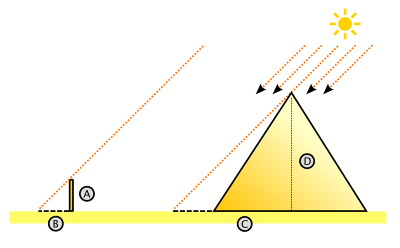
\includegraphics{cheops.png}\\
Fuente: Wikimedia Commons
\end{center}

Determine la altura de la pirámide a partir de esas medidas:

\begin{itemize}
  \item altura de la vara: 1.63m.
  \item sombra de la vara: 2m.
  \item longitud de la base de la pirámide: 230m.
  \item sombra de la pirámide: 65m.
\end{itemize}

\subsection{Ejercicio 5 (números constructibles)}

En este ejercicio, consideramos un segmento unidad sobre una hoja de papel y
queremos construir otra longitudes, utilizando sólo regla y compás.

\begin{center}
 \begin{tikzpicture}
   \draw (0,0)node[above]{$0$} -- (0.5,0)node[above]{$\vec{u}$} -- (1,0)node[above]{$1$};
   \draw (.8,.1) -- (1,0) -- (.8,-.1);
   \draw[fill=black] (0,0) circle(.05);
   \draw[fill=black] (1,0) circle(.05);
 \end{tikzpicture}
\end{center}

Indique cómo construir los ńumeros naturales $0, 1, 2, 3, 4, 5, \ldots$.

\begin{center}
 \begin{tikzpicture}
   \draw (0,0)node[above]{$0$} -- (1,0)node[above]{$1$}
   -- (2,0)node[above]{$2$} -- (3,0)node[above]{$3$}
   -- (4,0)node[above]{$\ldots$};
   \draw[fill=black] (0,0) circle(.05);
   \draw[fill=black] (1,0) circle(.05);
   \draw[fill=black] (2,0) circle(.05);
   \draw[fill=black] (3,0) circle(.05);
 \end{tikzpicture}
\end{center}

Indique cómo construir el eje ortogonal, de los números imaginarios puros:

\begin{center}
 \begin{tikzpicture}
   \draw (0,0)node[below]{$0$} -- (0.5,0)node[below]{$\vec{u}$} -- (1,0)node[below]{$1$};
   \draw (.8,.1) -- (1,0) -- (.8,-.1);
   \draw (0,0) -- (0,0.5)node[left]{$\vec{v}$} -- (0,1)node[left]{$i$};
   \draw (.1,.8) -- (0,1) -- (-.1,.8);
   \draw[fill=black] (0,0) circle(.05);
   \draw[fill=black] (1,0) circle(.05);
   \draw[fill=black] (0,1) circle(.05);
   \draw (0,.2) -- (.2,.2) -- (.2,0);
 \end{tikzpicture}
\end{center}

Ahora, consideramos dos enteros distinctos $p, q > 0$. Sea $D$ la recta (roja)
pasando por los puntos $(q,0)$ y $(0,1)$.
Indicar cómo trazar la recta (ázul) pasando por $(p,0)$ recta, paralela a $D$.

\begin{center}
 \begin{tikzpicture}
   \draw (0,0)node[below]{$0$} -- (0.5,0)node[below]{$\vec{u}$} -- (1,0)node[below]{$1$} -- (8,0);
   \draw (.8,.1) -- (1,0) -- (.8,-.1);
   \draw (0,0) -- (0,0.5)node[left]{$\vec{v}$} -- (0,1)node[left]{$i$} -- (0,5);
   \draw (.1,.8) -- (0,1) -- (-.1,.8);
   \draw[fill=black] (0,0) circle(.05);
   \draw[fill=black] (1,0) circle(.05);
   \draw[fill=black] (0,1) circle(.05);
   \draw (0,.2) -- (.2,.2) -- (.2,0);


   \draw[fill=black] (3,0) circle(.05) node[below]{$q$};
   \draw[fill=black] (7,0) circle(.05) node[below]{$p$};


   \draw[color=red] (-3,2) -- (6,-1);
   \draw[color=blue] (-3,3.333333333333333) -- (7,0);

 \end{tikzpicture}
\end{center}

¿Cual es el punto de intersección de esta recta ázul con el eje de 
de los números imaginarios puros? Deducir que todos los números racionales
son constructibles con regla y compás.

\section{Teorema de Pitágoras}

\subsection{Definición}

En un triángulo rectángulo, los catetos son los lados menores y la hipotenusa
es lado mayor.

\subsection{Teorema}

En todo triángulo rectángulo el cuadrado de la hipotenusa es igual a la suma de
los cuadrados de los catetos. 

\begin{center}
 \begin{tikzpicture}
   \draw (0,0) --
   (1.5,0)node[below]{$a$} -- (3,0) --
   (1.5,2)node[above right]{$c$} -- (0,4) --
   (0,2)node[left]{$b$} -- (0,0);
   \draw (0,.2) -- (.2,.2) -- (.2,0);
 \end{tikzpicture}
\end{center}

$$
a^2 + b^2 = c^2
$$

\subsection{Ejercicio 6}

Determine las longitudes $a,b,c$ de los lados de un triángulo rectángulo
(figura arriba), si

\begin{enumerate}
\item ¿$a = 12, b = 35$?
\item ¿$b = 56, c = 65$?
\item ¿$a = 11, c = 61$?
\end{enumerate}

\subsection{Ejercicio 7}

Consideramos la figura siguiente:

\begin{center}
 \begin{tikzpicture}

   \draw[color=black,fill=pink]
   (0,0) --
   (1.5,0)node[above]{$a$} -- (3,0) --
   (1.5,2)node[above right]{$c$} -- (0,4) --
   (0,2)node[right]{$b$} -- (0,0);

   \draw[color=black,fill=pink]
   (0,4) --
   (0,5.5)node[right]{$a$} -- (0,7) --
   (2,7)node[below]{$b$} -- (4,7) --
   (2,5.5)node[below right]{$c$} -- (0,4);

   \draw[color=black,fill=pink]
   (4,7) --
   (5.5,7)node[below]{$a$} -- (7,7) --
   (7,5)node[left]{$b$} -- (7,3) --
   (5.5,5)node[below left]{$c$} -- (4,7);

   \draw[color=black,fill=pink]
   (7,3) --
   (7,1.5)node[left]{$a$} -- (7,0) --
   (5.5,0)node[above]{$b$} -- (3,0) --
   (5,1.5)node[above left]{$c$} -- (7,3);

   \draw[color=blue]
   (0,0) -- (7,0) -- (7,7) -- (0,7) -- (0,0);

   \draw[color=green]
   (3,0) -- (7,3) -- (4,7) -- (0,4) -- (3,0);

 \end{tikzpicture}
\end{center}

Expresar en función de $a,b,c$:

\begin{itemize}
  \item La area $A$ del pequeño cuadrado (verde).
  \item La area $C$ del grán cuadrado (azul).
  \item La area rosa $B$ (cuatro triángulos rectángulos).
\end{itemize}

De la igualidad $C = A + B$ deduce el teorema de Pitágoras $c^2 = a^2 + b^2$.

\subsection{Ejercicio 8 (contruir una raíz cuadrada)}

Suponemos que tenemos una longitud unidad y otra longitud $x$.
Explique cómo obtener la figura siguiente con regla y compás:

\begin{center}
 \begin{tikzpicture}
   \draw[color=red, dashed] (10,0) arc (0:180:5);
   \draw(1.2,0) -- (1.2,.2) -- (1,.2);

   \draw(0,0) -- (0.5,0)node[below]{$1$} -- (1,0) --
   (5.5,0)node[below]{$x$} -- (10,0);
   \draw(1,0) -- (1,1.5)node[right]{$h$} -- (1,3);
   \draw(1,3) -- (5.5,1.5)node[above right]{$b$} -- (10,0);
   \draw(1,3) -- (.5,1.5)node[above left]{$a$} -- (0,0);

   \draw[color=blue]
   (0,-.5) -- (0,-1) -- (5,-1)node[below]{$c = 1 + x$} -- (10,-1) -- (10, -.5);
 \end{tikzpicture}
\end{center}

Un teorema de Tales dice que el triángulo inscrito en el círculo rojo,
de lados $a, b, c$ es rectángulo (ejercicio 6 del primer cápitulo).
Utilice el Teorema de Pitágoras sobre este
triángulo y dos otros para obtener la relación $h = \sqrt{x}$.

\subsection{Ejercicio 9}

Utilice las técnicas de los ejercicios 5 y 8 para construir
$x = \frac{17}{3}$, $p = \sqrt{17}$, $q = \sqrt{3}$, $\sqrt{x}$ y $\frac{p}{q}$.
Verifique geometricamente que 
%%
$$
\sqrt{\frac{17}{3}} = \frac{\sqrt{17}}{\sqrt{3}}
$$

\section{Soluciones de los ejercicios}

\subsection{Ejercicio 1}

Por ejemplo, dos triángulos $ABC$ y $AEF$ rectángulos en $A$ con
$1 = {AB} = {AC} = \frac{AE}{2} = \frac{AF}{2}$ tienen ángulos
$(90°, 45°, 45°)$ pero sus lados no son de misma longitud.

La recíproca es imposible: si $ABC$ y $DEF$ son congruentes, tenemos
$\frac{DE}{AB} = \frac{EF}{BC} = \frac{FD}{CA} = 1$.

\subsection{Ejercicio 2}

\begin{enumerate}
\item Tenemos
  $\widehat{C} = {180° - \widehat{A} - \widehat{B}} =
  {180° - \widehat{D} - \widehat{E}} = \widehat{F}$ y entonces
  los triángulos son semejantes.
\item Es fácil encontrar dos triángulos con $\widehat{A} = \widehat{D}$
  pero los otros ángulos que no coresponden.
\item Considerar por ejemplo $A = D$, $B = E$ y $AB = AC = DF$ pero
  $90° = \widehat{A} \neq \widehat{D} = 135°$.
\end{enumerate}

\subsection{Ejercicio 3 (Tales)}

\begin{enumerate}
\item Son ángulos opuestos por el vertice.
\item Son ángulos alternos.
\item Son ángulos corespondientes.
\end{enumerate}

De estas igualides de ángulos, vemos que $A_1B_1C_1$, $A_2B_2C_2$ y
$A_3B_3C_3$ son semejantes a $ABC$.

\subsection{Ejercicio 4 (pirámide de Keops)}

Los radios del sol son paralelas y por lo tanto podemos mover la vara para
que las extremidades de las sombras coincida al mismo punto. Podemos aplicar
el teorema de Tales:

$$
\frac{B}{C} = \frac{A}{D}
$$
%%
entonces $D = \frac{A C}{B} = \frac{1.63 \times
  \left(\frac{230}{2}+65\right)}{2} = 146.7m$

\subsection{Ejercicio 5 (números constructibles)}

Trazamos con la regla el eje pasando por los puntos $(0,0)$ y $(1,0)$. Con el
compás, podemos reportar la longitud del segmento inicial sobre este eje para
obtener los puntos $(2,0)$, $(3,0)$ etc que coresponden a los números naturales.

El eje ortogonal, de los ńumeros imaginarios puros es la mediatriz del segmento
$[-1,1]$. El punto $-1$ se contruye de la misma manera que los números
naturales. Con el compás, trazamos los círculos de centros $-1$ y $1$ y de
radio $2$. Se cortan en dos puntos sobre la mediatriz que podemos trazar con
la regla.

Con el compás, reportamos longitud del segmento inicial
sobre el eje de los ńumeros imaginarios puros para obtener el punto $(0,1)$ que
coresponde al ńumero complejo $i$. Con la regla, trazamos la recta roja pasando
por $(q,0)$ y $(0,1)$.

El círculo de centro $(p,0)$ y de radio $r=|p-q|$ corta la recta $D$ en
$Q_1={(q,0)}$ y otro punto $Q_2$. Con la técnica arriba, podemos trazar la
mediatriz de $[Q_1Q_2]$, que es la recta $D'$
ortogonal a $D$ pasando por ${(p,0)}$. El círculo de radio $1$ y centro
$(p,0)$ corta esta recta $D'$ en dos puntos $P_1, P_2$. De nuevo, trazamos
la mediatriz de $[P_1P_2]$: es la recta pasando por $(p,0)$ y paralela a
$D$, es decir la recta ázul.

La recta ázul intesecta el eje de los imaginarios puros en un punto
$(0,x)$ donde $x > 0$. Por el teorema de Tales, obtenemos
%%
$$
x = \frac{x}{1} = \frac{p}{q}
$$

Con el compás, podemos reportar esta longitud $x$ sobre el eje original para
obtener el punto $\left(\frac{p}{q}, 0 \right)$ corespondiente al racional
$\frac{p}{q}$. De la misma manera, obtenemos $-\frac{p}{q}$
Los casos $p = 0$ y $p = q$ coresponden a los puntos originales $0, 1$.
Entonces, podemos contruir todos los números racionales.

\subsection{Ejercicio 6}

\begin{enumerate}
\item $c = \sqrt{12^2 + 35^2} = 37$
\item $a = \sqrt{65^2 - 56^2} = 33$
\item $b = \sqrt{61^2 - 11^2} = 60$
\end{enumerate}

\subsection{Ejercicio 7}

\begin{itemize}
  \item $A = c^2$
  \item $C = \left(a+b\right)^2 = a^2 + {2ab} + b^2$
  \item $B = 4 \times \frac{ab}{2} = {2ab}$
\end{itemize}

Entonces $a^2 + b^2 = C - B = A = c^2$.

\subsection{Ejercicio 8 (contruir una raíz cuadrada)}

Trazamos una recta donde reportamos las longitudes $1$ y $x$ para obtener
un segmento de longitud $c = 1 + x$. Trazamos la mediatriz (ver ejercicio 5)
de este segmento para obtener el centro de círculo rojo que podemos dibujar con
el compás. Reportamos la unidad de referencia sobre el segmento para obtener
los puntos de coordenadas $0$ y $2$. La mediatriz del segmento formado por estos
puntos intersecta el círculo rojo para dar la nueva longitud $h$.

Las relaciones de Pitágoras se escriben:

$$c^2 = a^2 + b^2$$
$$a^2 = 1^2 + h^2$$
$$b^2 = x^2 + h^2$$

Entonces
${1^2+h^2 + x^2 + h^2} = a^2 + b^2 = c^2 = {(1+x)}^2 = 1^2+2x+x^2$,
$2h^2 = 2x$ y finalmente, $h = \sqrt{x}$.

\subsection{Ejercicio 9}

$x = \frac{17}{3}$ se obtene por la técnica del ejercicio 5.
$p = \sqrt{17}$, $q=\sqrt{3}$ y $\sqrt{x}$ se obtenen por la técnica del
ejercicio 8. Finalmente, $\frac{p}{q}$ se obtene como en el ejercicio 5
(no necesitamos que $p,q$ sean enteros para hacer la construción). Podemos
verificar que las longitudes $\sqrt{x}$ y $\frac{p}{q}$ son iguales.


\chapter{Reconoces las propiedades de los polígonos}

\section{Polígonos}

\subsection{Definición}

Wikipedia da las definiciones siguientes:

\begin{itemize}
\item Un polígono es una figura plana compuesta por una secuencia finita de
segmentos rectos consecutivos que cierran una región en el plano.
\item Un polígono es simple, si ningún par de aristas no consecutivas se corta.
  Equivalentemente, su frontera tiene un solo contorno.
\item Complejo, si dos de sus aristas no consecutivas se intersecan
\item Convexo, si tiene todos sus ángulos internos menores que 180º. O bien,
  si un segmento que une dos puntos cualesquiera del polígono yace en el
  interior de este.
\item Cóncavo, si al atravesarlo una recta puede cortarlo en más de dos puntos; es el que tiene uno o varios ángulos mayores que 180º.
\item Regular, si tiene todos sus lados iguales y todos sus ángulos iguales.
\item Un polígono con $n$ lado se llama un $n$-gono y para diferentes valor de
  $n$, dicemos que es un triángulo (3 lados), cuadrilátero (4 lados), pentágono
(5 lados), hexágono (6 lados), heptágono (7 lados), octógono (8 lados),
decágono (10 lados), dodecágono (12 lados) etc
\end{itemize}

\subsection{Ejercicio 1}

Indique si los figuras siguientes son polígonos.

\begin{enumerate}

\item
 \begin{tikzpicture}
   \draw (0,0) -- (1,0) -- (2,1) -- (1,2);
 \end{tikzpicture}

\item
  \begin{tikzpicture}
    \draw(1,1) --(0,0) -- (1,.5) -- (2,0) -- (1,1);
  \end{tikzpicture}

\item 
 \begin{tikzpicture}
   \draw (0,0) -- (1,-1) -- (2,0) arc (0:180:1);
 \end{tikzpicture}

\item 
 \begin{tikzpicture}
   \draw (0,0) node[left]{$(0,0)$} --
   (0,2)node[above left]{$(0,2)$} --
   (6,2)node[above left]{$(6,2)$} --
   (8,4)node[above right]{$(8,4)$} --
   (4,-2)node[below]{$(4,-2)$} --
   (2,1)node[above]{$(2,1)$} --
   (1,-.5)node[below]{$\left(\frac{8}{2^n}, {(-1)}^n \frac{4}{2^n} \right)$} --
   (.5,.25);
   \draw (.5,.25) -- (.25,-.125)[dashed];
 \end{tikzpicture}

\item 
  \begin{tikzpicture}
    \draw(0,0) --(2,0) -- (0,2) -- (2,2) -- (0,0);
  \end{tikzpicture}


\end{enumerate}

\subsection{Ejercicio 2}

Sean $A,B,C,D,E,G,G,H,I$ los puntos de coordenadas
$(0,0)$, $(1,0)$, $(2,0)$,
$(0,1)$, $(1,1)$, $(2,1)$,
$(0,2)$, $(1,2)$ y $(2,2)$. Dibuja y describe los polígonos siguientes:

\begin{enumerate}
  \item $AHFBD$
  \item $DBFH$
  \item $ABIHE$
  \item $DBFG$
  \item $BCIH$
\end{enumerate}

\subsection{Cuadriláteros}

Un cuadrilátero que tiene un par de lados paralelos es un trapezoide. Si
los lados opuestos son iguales y paralelos dos a dos, es llamado un
paralelogramo. Un paralelogramo con los cuatros lados paralelos es llamado
un rombo.

Un rectángulo tiene sus 4 ángulos de 90° y entonces es un
paralelogramo. Un cuadrado es un rectángulo con sus cuatro lados iguales y
por lo tanto es un cuadrilátero regular. 

\subsection{Ejercicio 3}

Dibuje:

\begin{enumerate}
\item un cuadrilátero simple convexo que no es un trapezoide.
\item un trapezoide que no es un paralelogramo.
\item un paralelogramo que es ni un rombo, ni un rectángulo.
\item un rombo que no es un cuadrado.
\item un rectángulo que no es un cuadrado.
\item un cuadrado.
\end{enumerate}

\section{Elementos y Propiedades}

\subsection{Definición}

Wikipedia da las definiciones siguientes:

\begin{itemize}
\item Lado: es cada uno de los segmentos que conforman el polígono.
\item Vértice: es el punto de intersección (punto de unión) de dos lados consecutivos.
\item Diagonal: es el segmento que une dos vértices no consecutivos.
\item Ángulo interior de un polígono simple: es el ángulo formado, internamente al polígono, por dos lados consecutivos.
\item Ángulo exterior de un polígono simple convexo: es el ángulo formado,
  externalmente al polígono,
  por un lado y la prolongación de un lado consecutivo.
\item Centro de un polígono regular: es el punto equidistante de todos los vértices y lados.
\item Ángulo central de un polígono regular:
  es el formado por dos segmentos de recta que parten del centro a los extremos
  de un lado.
\item Apotema de un polígono regular: es el segmento que une el centro del polígono con el centro de un lado; es perpendicular a dicho lado.
\end{itemize}

\subsection{Ejercicio 4}

Consideramos un polígono con $n \geq 3$ lados.

\begin{itemize}
\item ¿Cuantos vértices tiene?
\item ¿Cuantos diagonales tiene?
\item ¿Si es regular, cual es la medida de un ángulo central minimal?
  ¿Y la suma de esos ángulos centrales?
\end{itemize}

\subsection{Ejercicio 5}

\begin{itemize}
\item Represente sobre una figura los ángulos interiores y exteriores de
  un triángulo.
\item Recuerde cual es la suma de los ángulos interiores de un triángulo.
\item Deduzca la suma de los ángulos exteriores de un triángulo.
\item Sean $A, B, C$ tres vértices consecutivos de un $n$-gono
  simple convexo ($n \geq 4$).
  Represente sobre una figura los ángulos interiores y exteriores
  $\alpha, \beta, \gamma$
  en $A, B, C$.
\item Si retiramos el punto $B$, exprese la suma de los nuevos
  ángulos exteriores en $A$ y $C$.
\item Deduzca la suma de los ángulos exteriores de un poligóno simple convexo.
\item Exprese la suma de los angúlos interiores del $n-1$-gono ($B$ retirado).
  en función de la suma de los angúlos interiores del $n$-gono.
\item Deduzca la suma de los ángulos interior de un poligóno simple convexo.
\end{itemize}

\subsection{Ejercicio 6 (polígonos regulares)}

Utilice la regla y el compás para construir:

\begin{enumerate}
\item Un círculo $C$ de radio $R=4$.
\item Dos rectas ortogonales que se intersectan en el centro de $C$ (utilice
  la construcción de un mediatriz)
\item Un cuadrado inscrito en $C$.
\item Un polígono regular de lado $R$ y inscrito en $C$. ¿Cómo se llama?
\item Un triángulo equilátero inscrito en $C$.
  Sea $\beta$ un ángulo central de amplitud minimal.
\item La longitud $a=\sqrt{5} - 1$ (ver ejercicio 8 del capítulo III) y
  $b = R - a$.
\item El triángulo rectángulo con un lado menor $a = \sqrt{5} - 1$ y hipotenusa
  $R$. Sea $c$ el otro lado menor.
\item El triángulo rectángulo de catetos $b, c$. Sea $d$ su hipotenusa.
\item Un polígono regular de lado $d$ inscrito en $C$.
  ¿Cómo se llama? Sea $\alpha$ un ángulo central de amplitud minimal.
\item Dos polígonos regulares inscritos en $C$ de ángulos centrales minimales
  $\frac{\alpha}{2}$ y $\frac{\beta}{2}$ (construir las bisectrices de los
  ángulos $\alpha, \beta$). ¿Cómo se llaman?
\item Un octógono y hexadecágono ($16$-gono) regulares inscritos en $C$.
\item Un polígono regular inscrito en $C$ y
  ángulo central minimal $2 \alpha - \beta$. ¿Cómo se llama?
\end{enumerate}

\section{Perímetro y Área}

\subsection{Definición}

La suma de las longitudes los lados del polígono se llama el perímetro.
El tamaño de la región encerrada en el polígono se llama el área.

Por ejemplo, un rectángulo de lados $a,b$ tiene perímetro
$a+b+a+b=2{(a+b)}$ y área $a \times b$.

\begin{center}
 \begin{tikzpicture}
   \draw[color=red] (0,0) -- (2,0)node[below]{$a$} --
   (4,0) -- (4,1)node[right]{$b$} --
   (4,2) -- (2,2)node[above]{$a$} --
   (0,2) -- (0,1)node[left]{$b$} --
   (0,0);
 \end{tikzpicture}
\end{center}

\subsection{Ejercicio 7 (Cuadriláteros)}

\begin{enumerate}
\item
 ¿Cual es el perímetro y área de un cuadrado de lado $a$?

\begin{center}
 \begin{tikzpicture}
   \draw[color=red] (0,0) --
   (2,0) -- (2,1)node[right]{$a$} --
   (2,2) --
   (0,2) --
   (0,0);
 \end{tikzpicture}
\end{center}

\item Sean $a,b$ las longitudes de las diagonales de un rombo y $c$ la de
  un lado. Exprese el perímetro del rombo en función de $c$ y
  el área del rombo en función de $a,b$ (utilice el área del rectángulo ázul)?
  
\begin{center}
 \begin{tikzpicture}
   \draw (2.2,0) -- (2.2,.2) -- (2,.2);
   \draw (0,0) -- (4,0);
   \draw (2,-1) -- (2,1);
   \draw[dashed,color=blue] (0,-1) --
   (2,-1)node[below]{$b$} --
   (4,-1) -- (4,0)node[right]{$a$} -- (4,1) -- (0,1) -- (0,-1);
   \draw[color=red] (0,0) -- (2,-1) -- (4,0) -- (3,.5)node[above right]{$c$} --
   (2,1) -- (0,0);
 \end{tikzpicture}
\end{center}

\item Sean $a,b$ las longitudes de un lado de un paralelogramo y $h$ la
  distancia entre los dos lados paralelos de longitud $a$. 
  Exprese el perímetro del paralelogramo en función de $a,b$ y
  el área del paralelogramo en función de $a,h$.

\begin{center}
 \begin{tikzpicture}
   \draw[color=transparent,fill=pink] (0,0) -- (1,0) -- (1,1) -- (0,0);
   \draw[color=red] (0,0) -- (2,0)node[below]{$a$} --
   (4,0) -- (4.5,.5)node[right]{$b$} -- (5,1) -- (1,1) -- (0,0);
   \draw[dashed,color=blue] (1,0) -- (1,.5)node[right]{$h$} -- (1,1);
   \draw[dashed,color=blue] (4,0) -- (4,.5)node[left]{$h$} -- (4,1);
 \end{tikzpicture}
\end{center}

\item Sean $a,b$ las longitudes de los lados paralelos de un trapezoide y $h$ la
  distancia entre los dos lados.
  Exprese el área del trapezoide en función de $a,b,h$ (utilice el grán
  paralelogramo formado por dos copías del trapezoide).

\begin{center}
 \begin{tikzpicture}
   \begin{scope}[rotate around={180:(3.75,.5)}]
   \draw[dashed,color=red] (0,0) --
   (4,0) -- (3.5,1) -- (1,1) -- (0,0);
   \end{scope}

   \draw[color=red] (0,0) -- (2,0)node[below]{$a$} --
   (4,0) -- (3.5,1) -- (2.5,1)node[above]{$b$} -- (1,1) -- (0,0);

   \draw[dashed,color=blue] (1,0) -- (1,.5)node[right]{$h$} -- (1,1);
 \end{tikzpicture}
\end{center}

\begin{center}
 \begin{tikzpicture}
   \begin{scope}[rotate around={180:(5.5,.5)}]
   \draw[dashed,color=red] (0,0) --
   (4,0) -- (7,1) -- (1,1) -- (0,0);
   \end{scope}

   \draw[color=red] (0,0) -- (2,0)node[below]{$a$} --
   (4,0) -- (7,1) -- (2.5,1)node[above]{$b$} -- (1,1) -- (0,0);

   \draw[dashed,color=blue] (1,0) -- (1,.5)node[right]{$h$} -- (1,1);
 \end{tikzpicture}
\end{center}

\end{enumerate}

\subsection{Ejercicio 8 (Triángulo)}

\begin{enumerate}
\item Exprese el perímetro de un triángulo de lados $a,b,c$.
\item Formule expresiones del perímetro para un triángulo isósceles,
  equilátero, rectángulo o isósceles rectángulo.
\item Exprese el área de un triángulo de lado $a$ y altura $h$. 
\begin{center}
 \begin{tikzpicture}
   \draw[color=red]
   (0,0) -- (1.5,0)node[below]{$a$} -- (3,0) -- (4,3) -- (0,0);

   \begin{scope}[rotate around={180:(2,1.5)}]
   \draw[color=red,dashed]
   (0,0) -- (1.5,0) -- (3,0) -- (4,3) -- (0,0);
   \end{scope}
   \draw[color=blue,dashed](3,0)--(4,0)--(4,1.5)node[right]{$h$}--(4,3);
   \draw[color=blue](3.8,0)--(3.8,.2)--(4,.2);

   \begin{scope}[shift={(7,0)}]
     \draw[color=red]
     (0,0) -- (1.5,0)node[below]{$a$} -- (3,0) -- (2,3) -- (0,0);
     \begin{scope}[rotate around={180:(1,1.5)}]
     \draw[color=red,dashed]
     (0,0) -- (3,0) -- (2,3) -- (0,0);
     \end{scope}
     \draw[color=blue,dashed](2,0)--(2,1.5)node[right]{$h$}--(2,3);
   \draw[color=blue](1.8,0)--(1.8,.2)--(2,.2);
   \end{scope}
 \end{tikzpicture}
\end{center}
\item Formule expresiones del área para un triángulo rectángulo,
  isósceles rectángulo o equilátero.
 \end{enumerate}

\subsection{Ejercicio 9 (polígonos regulares, Arquímedes)}

\begin{enumerate}
\item Utilice la regla y el compás para construir: un círculo de centro $O$
  y radio $R$, el hexágono regular $ABCDEF$ de lado $R$ y inscrito en $C$,
  los radios ${OA}, {OB}, \ldots, {OF}$ y los seis apotemas del hexágono.
\item Exprese el périmetro, la longitud del apotema
   y el área del hexágono en función de $R$.
\item Consideramos el hexágono circunscrito a $C$, cuyos los apotemas
  son ${OA}, {OB}, \ldots, {OF}$. ¿Cual es su périmetro y
  área? Deduzca un aproximación del périmetro $P_C$ y área $A_C$ del círculo.
\item Suponemos que el périmetro del círculo es proporcional a la longitud
  de su radio $P_C = 2 \pi R$. Indique una aproximación de la constante $\pi$.
\item De manera general, si consideramos un polígono regular con $n \neq 6$
  lados de lado $l$ y apotema $h$, ¿Cuales son las formulas de périmetro y área?
\item Si tomamos $n$ muy largo, el perímetro del $n$-gono se acerca del
  perímetro del $P_C$, el apotema $h$ se acerca del radio $R$ y
  el área del $n$-gono se acerca del área $A_C$.
  Proponga una formula para el área $A_C$ del círculo en función de $R,\pi$.
\end{enumerate}

\section{Soluciones de los ejercicios}

\subsection{Ejercicio 1}

\begin{enumerate}

\item No (no cierra una región del plano).
\item Si (Polígono cóncavo)
\item No (tiene un segmento que no es recto)
\item No (tiene una infinitad de segmentos)
\item Si (Polígono complejo)
\end{enumerate}

\subsection{Ejercicio 2}

\begin{enumerate}
  \item Pentágono, complejo ($DB$ y $AH$ se intersectan).
  \item Cuadrilátero, simple, convexo, regular (cuadrado).
  \item Pentágono, simple, cóncavo (la amplitud de $\widehat{HEA}$ es
    más que 180°)
  \item Pentágono, simple, convexo ($DB \neq GF$).
\end{enumerate}

\subsection{Ejercicio 3}

\begin{enumerate}
\item 
 \begin{tikzpicture}
   \draw (0,0) -- (1,2) -- (2,0) -- (2,-1) -- (0,0);
 \end{tikzpicture}

\item 
 \begin{tikzpicture}
  \draw (0,0) -- (5,0) -- (4,1) -- (3,1) -- (0,0);
 \end{tikzpicture}
\item
 \begin{tikzpicture}
  \draw (0,0) -- (5,0) -- (7,2) -- (2,2) -- (0,0);
 \end{tikzpicture}
\item
 \begin{tikzpicture}
  \draw (0,0) -- (2,-1) -- (4,0) -- (2,1) -- (0,0);
 \end{tikzpicture}
\item 
 \begin{tikzpicture}
  \draw (0,0) -- (4,0) -- (4,2) -- (0,2) -- (0,0);
 \end{tikzpicture}
\item
  Por ejemplo
 \begin{tikzpicture}
  \draw (0,0) -- (2,0) -- (2,2) -- (0,2) -- (0,0);
 \end{tikzpicture}, o con otra orientación:
 \begin{tikzpicture}
  \draw (0,0) -- (1,-1) -- (2,0) -- (1,1) -- (0,0);
 \end{tikzpicture}
\end{enumerate}

\subsection{Ejercicio 4}

\begin{itemize}
\item Hay dos vértices para cada lados, y cada vértice apartene a dos lados
  entonces hay $\frac{2n}{2} = n$ vértices. Podemos también decir los
  vértices son exactamente los puntos de salida (o de llegada) de los
  lados, y entonces hay $n$ vértices. Por ejemplo, un triángulo tiene tres
  vértices, un cuadrilatero cuatro vértices etc
\item Para obtener un diagonal, elegimos un punto ($n$ posibilidades) y
  otro que no es conectado con el primer ($n-3$ posibilidades). Para cada
  diagonal hay dos posibilidades para el primer punto elegido y entonces
  hay $\frac{n{(n-3)}}{2}$ diagonales. Por ejemplo, un triángulo no tiene 
  diagonal, un cuadrilatero tiene dos diagonales, un pentágono tiene
  cinco diagonales etc
\item Una vuelta completa es 360°. Para un ángulo central (minimal), sólo
  es $\frac{1}{n}$ de una vuelta completa, es decir $\frac{360}{n}$. La suma
  de esos ángulos centrales es 360°.
\end{itemize}

\subsection{Ejercicio 5}

Los ángulos rojos son los ángulos interiores y
los ángulos azules son los ángulos exteriores. La suma de los ángulos interiores
es $x+y+z=180°$.
Además, cada par de ángulo interior/exterior coresponde a
ángulos suplementarios. Entonces la suma de los ángulos exteriores es
${(180° - x)} + {(180° - y)} + {(180° - z)} = 3\times180° - {(x+y+z)} = 360°$.

\begin{center}
 \begin{tikzpicture}
   \draw (0,0) -- (3,0) -- (2,1) -- (0,0);
   \draw[dashed] (3,0) -- (4,-1);
   \draw[dashed] (2,1) -- (4,2);
   \draw[dashed] (0,0) -- (-2,0);

   \draw[color=red](.5,0) arc(0:26:.5) node(A){};
   \draw[color=blue](A) arc(26:180:.5);

   \draw[color=blue](2.5,0) arc(180:316:.5);
   \draw[color=red](2.5,0) arc(180:136:.5);

   \draw[color=blue](2.449397023149583,1.219185573394538) arc(26:-43:.5) node(B){};
   \draw[color=red](B) arc(-43:-152:.5);

 \end{tikzpicture}
\end{center}

Los ángulos rojos son los ángulos interiores y los
ángulos azules son los ángulos exteriores.

\begin{center}
 \begin{tikzpicture}
   \draw (0,-2)node[below]{$\vdots$} -- (0,0)node[above left]{$C$} -- (2,1)
   node[above]{$B$} -- (3,0)node[above right]{$A$} --
   (3,-2)node[below]{$\vdots$};
   \draw[dashed] (3,0) -- (4,-1);
   \draw[dashed] (2,1) -- (4,2);
   \draw[dashed] (0,0) -- (0,2);

   \draw[color=red](0,-.5) arc(-90:26:.5) node(A){};
   \draw[color=blue](A) arc(26:90:.5) node[above right]{$\gamma$};

   \draw[color=blue](3,-.5)node[below right]{$\alpha$} arc(270:316:.5);
   \draw[color=red](3,-.5) arc(270:136:.5);

   \draw[color=blue](2.449397023149583,1.219185573394538)
   node[below right]{$\beta$} arc(26:-43:.5) node(B){};
   \draw[color=red](B) arc(-43:-152:.5);

   \draw[dashed,color=green] (0,0) -- (3,0);

 \end{tikzpicture}
\end{center}

Si retiramos el punto $B$, la amplitud del ángulo exterior en $A$ se vuelve
$\alpha + \widehat{CAB}$ y la amplitud del ángulo exterior en $C$ se vuelve
$\gamma + \widehat{BCA}$. Entonces la suma de estes dos ángulos es
$\alpha + \gamma + \widehat{CAB} + \widehat{BCA} =
\alpha + \gamma + {(180° - \widehat{ABC})} = \alpha+\beta+\gamma$.
Por lo tanto, la suma de los ángulos exteriores de un
$n$-gono es la misma que la suma de los angúlos interiores de un $n-1$-gono,
de un $n-2$-gono, $n-3$-gono... y finalmente de un triángulo es decir 360°.

De la misma manera, para obtener la suma de los angúlos interiores en el
$n-1$-gono a partir de la suma del $n$-gono,
restamos el ángulo interior $\widehat{ABC}$,
restamos $\widehat{CAB}$ del ángulo interior en $A$ y
restamos $\widehat{BCA}$ del ángulo interior en $C$. Entonces restamos
$\widehat{ABC}+\widehat{CAB}+\widehat{BCA}=180°$. Al final,
la suma de los ángulos interiores de un triángulo es $180°$, la de un
cuadrado $180+180=360°$, ... y la de un $n$-gono $180\times {(n-2)}$°.

Note que las definiciones y resultados pueden ser generalizados a polígonos
que no son simple o convexo.

\subsection{Ejercicio 6 (polígonos regulares)}

Trazamos el círculo $C$ (azul) con el compás. Con la regla trazamos una recta
pasando por el centro de $C$. Cómo en el ejercicio 5 del capítulo III,
trazamos la recta ortogonal pasando por $C$. Los puntos de interseción de estas
rectas con el círculo $C$ son los cuatros vértice de un cuadrado inscrito en
$C$ (rojo). 

Trazamos con el compás el círculo de centro un punto de $C$ y radio $R$.
Intersecta $C$ en un nuevo punto. Si repetamos esta operación otras veces,
obtenemos un hexágono regular inscrito en $C$ (verde). Tomando un punto sobre
dos de este hexágono, obetemos un triángulo equilátero inscrito en $C$
(naranja).

\begin{center}
\begin{tikzpicture}
  \draw (0,0) circle(4)[color=blue];
  \draw[fill=black] (0,0) circle(.05)[color=blue];
  \draw (-5,0) -- (5,0)[dashed,color=red];
  \draw (0,-5) -- (0,5)[dashed,color=red];
  \draw (4,0) -- (0,4) -- (-4,0) -- (0,-4) -- (4,0)[color=red];
  \draw (4,4) arc(90:180:4)[dashed,color=green];
  \draw (4,0) -- (2,3.464101615137754) -- (-2,3.464101615137754) --
  (-4,0) -- (-2,-3.464101615137754) -- (2,-3.464101615137754) -- (4,0)
        [color=green];
  \draw (4,0) -- (-2,3.464101615137754) -- (-2,-3.464101615137754) -- (4,0)
        [color=orange];
\end{tikzpicture}
\end{center}

Cómo en el ejercicio 8 del capítulo III, podemos construir la longitud
$\sqrt{5}$ y
entonces $a = \sqrt{5} - 1$ y $b = R - a$. Utilizamos la técnica de la mediatriz
para construir los dos triángulos rectángulos. Repetamos la longitud $d$ con
el compás para obtener un pentágono regular inscrito en $C$ (verde).

\begin{center}
\begin{tikzpicture}
  \draw (0,0) circle(4)[color=blue];
  \draw[fill=black] (0,0) circle(.05)[color=blue];
  \draw (-5,0) -- (5,0)[dashed,color=red];
  \draw (0,-5) -- (0,5)[dashed,color=red];
  \draw[fill=black] (2.23606797749979,0) circle(.05);
  \draw[dashed, color=orange] (2.23606797749979,0) -- (2.23606797749979,-.2) --
  (1.78606797749979,-.2) node[below]{$1$} -- (1.23606797749979,-.2) --
  (1.23606797749979,0);
  \draw[fill=black] (1.23606797749979,0) circle(.05);
  \draw[color=green](0,0) -- (.6,0) node[above]{$a$} --
  (1.23606797749979, 0) -- 
  (1.23606797749979, 1.9)node[right]{$c$} -- 
  (1.23606797749979,3.804226065180614) --
  (.6, 1.9)node[above left]{$R$} -- (0,0);
  \draw[color=green] (1.23606797749979, 0) --
  (2.5,0) node[above]{$b$} -- (4,0) -- 
  (2.618033988749894,1.902113032590307)node[above right]{$d$} --
  (1.23606797749979,3.804226065180614);
  \draw[color=green](1.43606797749979,0) --
  (1.43606797749979,.2) -- (1.23606797749979,.2);
  \draw[color=green]
  (1.23606797749979,3.804226065180614) --
  (-3.236067977499789,2.351141009169893) --
  (-3.23606797749979,-2.351141009169892) --
  (1.23606797749979,-3.804226065180614) -- (4, 0);
  \draw(2.23606797749979,0) -- (3,-1) node[below]{$(\sqrt{5},0)$};

\end{tikzpicture}
\end{center}

Construyendo las mediatrices de los lados del pentágono (es decir las
bisecrices de sus ángulos centrales) obtenemos un decágono regular (naranja)
inscrito en $C$. De la misma manera, a partir del cuadrado y hexágono
obtenemos octógono y dodecágono regulares inscritos en $C$. Y a partir del
octógono, obtenemos un hexadecágono.

\begin{center}
\begin{tikzpicture}
  \draw (0,0) circle(4)[color=blue];
  \draw[fill=black] (0,0) circle(.05)[color=blue];
  \draw[color=green]
  (1.23606797749979,3.804226065180614) --
  (-3.236067977499789,2.351141009169893) --
  (-3.23606797749979,-2.351141009169892) --
  (1.23606797749979,-3.804226065180614) -- (4, 0) --
  (1.23606797749979,3.804226065180614);
  \draw[dashed,color=red] (0,0) -- (4,0);
  \draw[dashed,color=red] (0,0) -- (1.23606797749979,3.804226065180614);
  \draw[dashed,color=orange] (0,0) -- (3.23606797749979,2.351141009169892);
  \draw[color=orange]
  (4,0) --
  (3.23606797749979,2.351141009169892) --
  (1.23606797749979,3.804226065180614) --
  (-1.23606797749979,3.804226065180614) --
  (-3.236067977499789,2.351141009169893) --
  (-4,0) --
  (-3.23606797749979,-2.351141009169892) --
  (-1.23606797749979,-3.804226065180614) --
  (1.23606797749979,-3.804226065180614) --
  (3.236067977499789,-2.351141009169893) --
  (4, 0);

\end{tikzpicture}
\end{center}

Utilizando las construciones del triángulo equilátero y del pentágono regular,
podemos construir el ángulo $2\alpha - \beta =
2 \times \frac{360}{5} - \frac{360}{3} = \frac{360}{15}$. Eso nos permite
construir un pentadecágono ($15$-gono) regular inscrito en $C$.

\begin{center}
\begin{tikzpicture}
  \draw (0,0) circle(4)[color=blue];
  \draw[fill=black] (0,0) circle(.05)[color=blue];
  \draw[color=green]
  (4, 0) --
  (1.23606797749979,3.804226065180614) --
  (-3.236067977499789,2.351141009169893) --
  (-3.23606797749979,-2.351141009169892) --
  (1.23606797749979,-3.804226065180614) -- 
  (4,0);
  \draw[color=orange]
  (-3.236067977499789,2.351141009169893) -- (3.654181830570403,1.6269465723032)
  -- (-0.41811385307061,-3.978087581473093) --
  (-3.236067977499789,2.351141009169893);
  \draw[dashed,color=red]
  (4,0) -- (0,0) -- (-3.236067977499789,2.351141009169893);
  \draw[dashed,color=red]
  (0,0) -- (3.654181830570403,1.6269465723032);
  \draw[color=green] (.5,0) arc (0:72:.5) node[above right]{$2\alpha$} 
  arc (72:144:.5);
  \draw[color=orange] (1.370318186463901,0.6101049646137) arc (24:100:1.5)
  node[above right]{$\beta$} arc (100:144:1.5);

  \draw[color=purple] (2,0) arc (0:12:2)
  node[right]{$2\alpha-\beta$} arc (12:24:2);

  \draw[color=purple] (4,0) -- 
  (3.654181830570403,1.6269465723032)--
  (2.676522425435433,2.972579301909576) --
  (1.236067977499789,3.804226065180614) --
  (-0.41811385307061,3.978087581473093) --
  (-2.0,3.464101615137754) --
  (-3.236067977499789,2.351141009169893) --
  (-3.912590402935222,0.83164676327103) --
  (-3.912590402935222,-0.83164676327103) --
  (-3.236067977499789,-2.351141009169893) --
  (-2.0,-3.464101615137754) --
  (-0.41811385307061,-3.978087581473093) --
  (1.236067977499789,-3.804226065180614) --
  (2.676522425435433,-2.972579301909576) --
  (3.654181830570403,-1.6269465723032) --
  (4,0);
\end{tikzpicture}
\end{center}

En este ejercicio, hemos obtenido todos los $n$-gonos regulares que es
posible contruir con regla y compás, para $n \leq 16$. Gaus dio una construción
del heptadecágono regular ($n=17$ lados).

\subsection{Ejercicio 7 (Cuadriláteros)}

\begin{enumerate}
\item Un cuadrado de lado $a$ tiene perímetro $4a$ y área $a^2$. 
\item El perímetro del rombo es $4c$ y
  su areá es la mitad del rectángulo ázul, es decir $\frac{ab}{2}$.
\item La formula del perímetro es la misma que la del rectángylo: $2{(a+b)}$.
  Podemos cortar el triángulo rosa y mover esta parte para obtener un
  rectángulo de lados $a,h$ de misma área: $a \times h$.
\item El área del trapezoide es la mitad del paralelogramo:
  $\frac{{(a+b)} \times h}{2}$.
\end{enumerate}

\subsection{Ejercicio 8 (Triángulo)}

\begin{enumerate}
\item $a+b+c$
\item $3a$ (equilátero de lado $a$), $a+2b$ (isósceles de lado $a,b,b$)
  $a+b+\sqrt{a^2+b^2}$ (rectángulo de lados menores $a,b$),
  ${(2+\sqrt{2})}a$ (rectángulo isósceles de lados menor $a$).
\item Es la mitad del paralelogramo en la figura: $\frac{a \times h}{2}$.
\item Un triángulo rectángulo de lado menores $a,b$ (respectivamente
  rectángulo isósceles de lado menor $a$) es la mitad de un rectángulo de lado
  $a,b$ ((respectivamente de un cuadrado de lado $a$) y obtenemos
  $\frac{ab}{2}$ y $\frac{a^2}{2}$. En la formula general, $a$ es un lado menor
  y la altura $h$ el otro lado menor.

  Para un triángulo equilátero de lado $a$, el teorema de pitágoras da
  $h = \sqrt{a^2 - \left(\frac{a}{2}\right)^2} = \frac{\sqrt{3}}{2} a$ y
  entonces el área es $\frac{\sqrt{3}}{4} a^2$.
  
\end{enumerate}

\subsection{Ejercicio 9 (polígonos regulares, Arquímedes)}

\begin{enumerate}
\item Ver el Ejercicio 6:

\begin{center}
\begin{tikzpicture}
  \draw (0,0) circle(4)[color=blue];
  \draw[fill=black] (0,0) circle(.05)[color=blue] node[above right]{$O$};

  \draw (-4,0) -- (4,0)[color=green];
  \draw (0,-3.464101615137754) -- (0,3.464101615137754)[dashed,color=red];

  \begin{scope}[rotate around={60:(0,0)}]
  \draw (-4,0) -- (4,0)[color=green];
  \draw (0,-3.464101615137754) -- (0,3.464101615137754)[dashed,color=red];
  \end{scope}

  \begin{scope}[rotate around={120:(0,0)}]
  \draw (-4,0) -- (4,0)[color=green];
  \draw (0,-3.464101615137754) -- (0,3.464101615137754)[dashed,color=red];
  \end{scope}

  \draw (4,4) arc(90:180:4)[dashed,color=green];
  \draw (4,0) node[right]{$A$}
  -- (2,3.464101615137754)  node[above right]{$B$}
  -- (-2,3.464101615137754)  node[above left]{$C$}
  -- (-4,0)  node[left]{$D$}
  -- (-2,-3.464101615137754) node[below left]{$E$}
  -- (2,-3.464101615137754) node[below]{$F$}
  -- (4,0) [color=green];


\end{tikzpicture}
\end{center}


\item El hexágono tiene $6$ lados de longitud $R$ y entonces el
  périmetro es $6R$. Cómo en el ejercicio 8, 
  la longitud del apotema es $\frac{\sqrt{3}}{2} R$ y 
  la área es del hexágono
  es $6 \frac{\sqrt{3}}{4} R^2 = \frac{3 \sqrt{3}}{2} R^2$.
\item Eso es un hexágono de radio
  ${\frac{2}{\sqrt{3}} R}={\frac{2\sqrt{3}}{3} R}$ y entonces
  de périmetro $4 \sqrt{3} R$ y área $2 \sqrt{3} R^2$.
  Entonces $6R \leq P_C \leq 4 \sqrt{3} R$ y
  $\frac{3 \sqrt{3}}{2} R^2 \leq A_C \leq 2 \sqrt{3} R^2$.
\item $3 = \frac{6R}{2R} \leq \pi \leq \frac{4 \sqrt{3} R}{2R} = 2\sqrt{3} \approx 3.464101615137754$.
  Arquímedes utilizó $96$-gonos para obtener una mejor approximación
  $3.1408 \approx \frac{310}{71} \leq \pi \leq \frac{31}{7} \approx 3.1429$.
\item Si el polígono tiene $n$ lados de longitud $l$, su perímetro es $nl$.
  Su área se compone de $n$ tríangulos de lado $l$ y altura $h$ entonces
  es $n \frac{l \times h}{2} = \frac{nlh}{2}$.

\item El perímetro $nl$ se acerca de $P_C = 2 \pi R$, la altura $h$ se acerca
  de $R$. Entonces el área del polígono se acerca de
  $\frac{2 \pi R \times R}{2} = \pi R^2$. En efecto, podemos mostrar que
  el área de un círculo de radio $R$ es $A_C = \pi R^2$.
\end{enumerate}

\chapter{Realizas transformaciones algebraicas II}

\section{Técnicas de factorización}

\subsection*{Resumen}

Ya hemos visto productos notables (factor común, cuadrado de un binomio,
cubo de un binomio, binomios conjugados). Otra técnica para factorizar un
polinomio es encontra un ``cero trivial'' $a$, para deducir un factor
$X - a$. Podemos también tratar escribir el polinomio como un producto. Por
ejemplo si queremos factorizar el polinomio $P = x^2 - 3x + 2$ como un
producto de dos factores lineales,
${(x - x_1)}{(x-x_2)} = x^2 - {(x_1+x_2)}x + x_1 x_2$ y podemos poner
$x_1 = 1$ y $x_2 = 2$.

\subsection*{Ejercico 1}

\begin{enumerate}
\item Factorizar $X^2 + 34X + 289$ (producto notable)

\item Sea $P = 6 Y^2 + Y -35$. Factorizar $P$ como un producto
  ${(aY + b)}{(cY + d)}$ donde $a, b, c, d$ son enteros

\item Sea $P = X^3+33X^2+255x-289$. Calcular $P$ en $x = -1, 0, 1$. Factorizar
  $P$.
\end{enumerate}

\subsection*{Ejercico 2}

Consideramos $P = Z^2 + \left(\frac{5}{2} - \sqrt{3}\right) Z -
\frac{5 \sqrt{3}}{2}$.

\begin{enumerate}
\item Developar $Q = \left( Z + \frac{5}{4} - \frac{\sqrt{3}}{2} \right)^2$
\item Mostrar que $k = Q - P$ es una constante.
\item Encontrar enteros $a, b$ tales que
  $\left(\frac{a \sqrt{3} + b}{4}\right)^2 = k$.
\item Utilizar un producto notable para factorizar $P = Q - k$.
\end{enumerate}

\section{Expresiones racionales y división de polinomio}

\subsection*{Resumen}

Una expresión racional se escribe como una fración de dos polinomios
$\frac{P}{Q}$. Si $P, Q$ tienen un factor comúm, podemos simplifiar la fracción
por este factor.

Podemos también definir la división de dos polinomios $A$ 
y $B$ de la misma manera como la división Euclídea de dos enteros:

$$A = B Q + R$$

donde el cociente $Q$ y el resto $R$ son únicos polinomios tales que el grado
de $R$ es estrictamente menor que el grado de $B$. En particular, podemos
escribir la egualidad de expresiónes racionales:

$$\frac{A}{B} = Q + \frac{R}{B}$$

\subsection*{Ejemplo}

\begin{enumerate}
\item $\frac{X^3-1}{X^2-X}$ es una expresión racional. El numerador es
  $X^3 - 1 = {(X-1)}{(X^2+X+1)}$ y el denominador $X^2+X = X{(X-1)}$. Entonces
  podemos simplificar la expresión racional como $\frac{X^2+X+1}{X}$.
\item Tenemos $X^2+X+1 = Q X + R$ donde $Q = X + 1$ y $R = 1$. El grado de $R$
  es estrictamente menor que el grado de $X$ entonces eso es la divisíon de
  $X^2+X+1$ por $X$. La expresión racional precedente puede ser escrita
  $X+1 + \frac{1}{X}$.
\end{enumerate}

\subsection*{Ejercicio 3}

Efectuar la división de los polinomios siguientes:

\begin{enumerate}
\item $X^5+2X^3-X^2+X+2$ por $X^2+2$
\item $X^8-2X^7+X^6+X^2-4X+3$ por $X^7 - X^6$
\item $X^5+16X^4+64X^3-X^2-16X-64$ y $X^4+17X^3+80X^2+64X$
\end{enumerate}

\subsection*{Ejercicio 4}

Simplificar las expresión racionales siguientes:

\begin{enumerate}
\item $\frac{X^5+2X^3-X^2+X+2}{X^2+2}$
\item $\frac{X^8-2X^7+X^6+X^2-4X+3}{X^7 - X^6}$
\item $\frac{X^5+16X^4+64X^3-X^2-16X-64}{X^4+17X^3+80X^2+64X}$
  (al final, utilizar $X - 1 = 2X - {(X+1)}$)
\end{enumerate}

\section{Soluciones de los ejercicios}

\subsection*{Ejercicio 1}

\begin{enumerate}
\item ${(X+17)}^2$

\item 
  ${(aY + b)}{(cY + d)} = acY^2 + {(ad+bc)}Y + bd = 6 Y^2 + Y -35$.
  Tratamos encontrar $a,b,c,d$ enteros tales que
  $ac = 6$, $ad+bc = 1$ y $bd= -35$. Podemos suponer $c \geq 0$ (sino, podemos
  cambiar el signo de todos los coeficientes y no cambia las egualidades).
  Por la primera relación, $c \in \{ 1, 2, 3, 6 \}$. Podemos también suponer
  que ${|c|} \leq {|a|}$ (sino, podemos intercambiar los dos factores). Entonces
  $c = 1$ (y $a=6$) o $c = 2$ (y $a=3$). Para cada caso, tratamos las
  posibilidades por $bd = -35 = -1 \times 5 \times 7$ y
  $ad+bc = 1$. Encontramos $c = 2$, $a=3$, $b=-7$ y $d=5$.
  Por consequencia, $P = {(2x+5)}{(3x-7)}$.

\item $P(0) = -289$, $P(-1) = -1 -33 -255 -289 = -512$,
  $P(1) = 1 + 33 + 255 - 289 = 0$. Tratamos escribir
  $P = {(X - 1)}{(X^2 + bX + c)} = X^3 + {(b - 1)}X^2 + {(c - b)}X - c$.
  Podemos tomar $c = 289$ y $b = 34$. Entonces
  $P = {(X-1)}{(X^2 + 34X + 289)} = {(X-1)}{(X+17)}^2$.
\end{enumerate}

\subsection*{Ejercico 2}

\begin{enumerate}
\item $Q = Z^2 + \left(\frac{5}{2} - \sqrt{3}\right) Z + \frac{37}{16} - \frac{5 \sqrt{3}}{4}$
\item Encontramos $k = Q - P = \frac{20\sqrt{3} + 37}{16}$.
\item Debemos resolver $3a^2 + b^2 = 37$ y $2ab=20$. Tratamos dividores de 20
  y finalmente $a = 2$ y $b = 5$ conviene.
\item $P = Q - k = \left( Z + \frac{5}{4} - \frac{\sqrt{3}}{2} \right)^2 -
  \left(\frac{2 \sqrt{3} + 5}{4} \right)^2$. Utilizamos la ley de los
  binomios conjugados:

  $$P = \left( Z + \frac{5}{4} - \frac{\sqrt{3}}{2} 
  - \frac{2 \sqrt{3} + 5}{4}
  \right) \left( Z + \frac{5}{4} - \frac{\sqrt{3}}{2} 
  + \frac{2 \sqrt{3} + 5}{4}
  \right) =
  \left( Z - \sqrt{3} \right) \left( Z + \frac{5}{2} \right)$$
\end{enumerate}

\subsection*{Ejercicio 3}

\begin{enumerate}
\item $Q = X^3-1, R = X + 4$
\item $Q = X - 1, R = X^2 -4X + 3$
\item $Q = X - 1, R = X^3+15X^2+48X - 64$
\end{enumerate}

\subsection*{Ejercicio 4}

\begin{enumerate}
\item Por el precedente ejercicio, se escribe $X^3 - 1 + \frac{X+4}{X^2+2}$.
\item Por el precedente ejercicio, se escribe
  $X-1 + \frac{X^2-4X+3}{X^7-X^6}$. En la fracción,
  $1$ es un cero trivial del numerador y del numerador entonces $X-1$ es un
  factor común y finalmente obtenemos
  $X-1 + \frac{1}{X^5} - \frac{3}{X^6}$
\item Por el precedente ejercicio, se escribe
  $X - 1 + \frac{X^3+15X^2+48X-64}{X^4+17X^3+80X^2+64X}$. En la fracción, $1$ es
  un cero trivial del numerador y $0, -1$ ceros triviales del denominador.
  Factorizando cada uno, nos damos cuenta de que $(X+8)^2$ es un factor común
  y finalmente obtenemos $X - 1 + \frac{X-1}{X{(X+1)}} = 
  X - 1 + \frac{2}{X+1} - \frac{1}{X}$.
\end{enumerate}

\chapter{Describes las relaciones trigonométricas para resolver triángulos rectángulos}

\section{Sistema sexagesimal y circular}

\subsection{Definicíon}

Para medir un ángulo, un grado representa $\frac{1}{360}$ de una
circunferiancia. Un minuto representa $\frac{1}{60}$ de un grado y un segundo
$\frac{1}{60}$ de un minuto. Por ejemplo un ángulo de 1° 9' 18'' representa
$\frac{1}{360} + 9 \times \frac{1}{360 \times 60} + 18 \times \frac{360 \times 60 \times 60} = \frac{77}{24000}$ de una circunferiancia. Eso es llamado el
sistema sexagesimal.

En ciencia, el sistema circular es más utilizado. Es definido tal que si un
ángulo $\alpha$ mide un radián, la longitud del arco corespondiente en
un círculo de radio $R$ sólo es $\alpha \times R$. Entonces, la medida de una
circunferencia corresponde a $2\pi \text{rad}$, la medida de una
semicircunferencia es $\pi \text{rad}$, la medida de un cuarto de la
circunferencia es $\frac{\pi}{2} \text{rad}$ etc

\subsection{Ejercicio 1}

\begin{enumerate}
\item Indique la valor en grado, minuto y segundo de un ángulo de $15.75$° y
  y $78.51$°.
\item Indique una approximación la medida en grado/minuto/segundo de un ángulo
  de 1 radián.
\item Exprese en función de $\pi$, la medida en radián de los ángulos de
  30°, 45°, 60°, 90°, 135°, 180°, 270° y 360°.
\item Exprese la formula de la área de un sector de $\alpha$ radianes para
  un círculo de radio $R$.
\end{enumerate}

\section{Funciones trigonométricas}

\subsection{Definicíon}

Consideramos un triángulo rectangulo y $\alpha$ la medida de un ángulo en
radián ($0 \leq \alpha < \frac{\pi}{2}$).

\begin{center}
 \begin{tikzpicture}
   \draw[color=blue] (0,0) -- (1.5,0)node[below]{adyacente} -- (3,0);
   \draw[color=green] (3,0) -- (3,2)node[right]{opuesto} -- (3,4);
   \draw[color=red] (3,4) -- (1.5,2)node[above left]{hipotenusa} -- (0,0);
   \draw (2.8,0) -- (2.8,.2) -- (3,.2);
   \draw[color=orange] (0.5,0) arc(0:25:.5) node[above right]{$\alpha$}
   arc(25:53.13010235415599:.5);
   \draw[fill=black] (3,4) node[above right]{$M$} circle(.05);
 \end{tikzpicture}
\end{center}

Esos ángulos recto y $\alpha$ determinan la clase de semejanza del
triángulo y por lo tanto los cocientes siguientes:

$$
\sin \alpha = \frac{\color{green}{\text{opuesto}}}
{\text{\color{red}{\text{hipotenusa}}}}
$$
%%
$$
\cos \alpha = \frac{\color{blue}{\text{adyacente}}}
{\text{\color{red}{\text{hipotenusa}}}}
$$
%%
$$
\tan \alpha = \frac{\color{green}{\text{opuesto}}}
{\text{\color{blue}{\text{adyacente}}}}
$$

Cuando $\alpha$ se acerca del ángulo recto $\frac{\pi}{2}$, la longitud
del lado opuesto se acerca de la longitud del hipotenusa y la longitud
del lado adyacente se acerca de 0. Por lo tanto, definimos
%%
$$
\cos \frac{\pi}{2} = 0
$$
%%
$$
\sin \frac{\pi}{2} = 1
$$
%%
pero no definimos $\tan$ en $\frac{\pi}{2}$, porque el cociente
$\frac{\color{green}{\text{opuesto}}}
{\text{\color{blue}{\text{adyacente}}}}$ se vuelve más en más grande cuando
$\alpha$ se acerca de $\frac{\pi}{2}$.

Podemos genaralizar las formulas precedientes si utilizamos valores
relativas para
$\color{green}{\text{opuesto}}$ y ${\text{\color{blue}{\text{adyacente}}}}$
según las coordenadas del vértice $M$ opuesto al ángulo $\alpha$:

$$\cos{(-\alpha)} = \cos{(\alpha)}$$
$$\sin{(-\alpha)} = -\sin{(\alpha)}$$
$$\tan{(-\alpha)} = -\tan{(\alpha)}$$
$$\cos{(\pi-\alpha)} = -\cos{(\alpha)}$$
$$\sin{(\pi-\alpha)} = \sin{(\alpha)}$$
$$\tan{(\pi-\alpha)} = -\tan{(\alpha)}$$

Finalmente hacer una vuelta $2\pi$ no debe cambiar los cocientos y entonces
la funciones deben ser periódicas (el ejercico 3 da un mejor resultado para
tangente):

$$\cos{(\alpha+2\pi)} = \cos{(\alpha)}$$
$$\sin{(\alpha+2\pi)} = \sin{(\alpha)}$$
$$\tan{(\alpha+2\pi)} = \tan{(\alpha)}$$

Esas formulas definen las funciones seno y coseno para todo
$\alpha \in \mathbb R$ y la función tangente sobre todo
$\alpha \in \left]{-\frac{\pi}{2} + k\pi}, {\frac{\pi}{2} +k\pi} \right[$
para $k \in \mathbb Z$. 

\subsection{Ejercicio 2}

\begin{enumerate}
  \item ¿Cuál es el seno, coseno y tangente de $\alpha=0$?
  \item Determine el ángulo $\alpha$ en un triángulo rectángulo isoceles
    así que el seno, coseno y tangente de $\alpha$.
  \item Consideramos un triángulo equilatero $ABC$ y sea $D$ el medio
    de $[BC]$. Muestre que $ABD$ es rectángulo en $D$ y determine sus
    ángulos $\widehat{A}$ y $\widehat{B}$ así que sus seno, coseno y
    tangente de los ángulos.
  \item Expresar los seno, coseno y tangente de $\frac{\pi}{6}$ y
    $\frac{\pi}{4}$ así que de sus múltiplos.
\end{enumerate}

\subsection{Ejercicio 3}

Muestre las igualidas siguientes para $0 \leq \alpha < \frac{\pi}{2}$:

\begin{enumerate}
\item Utilice $\alpha + \pi = -\left(\pi-\alpha\right) + 2\pi$ para determinar
  $\cos\left(\alpha+\pi\right)$ y $\sin\left(\alpha+\pi\right)$.
\item $\tan \alpha = \frac{\sin \alpha}{\cos \alpha}$. Deduzca que 
  $\tan \left(\alpha+\pi\right)$.
\item $\left(\sin \alpha\right)^2 + \left(\cos \alpha\right)^2 = 1$
\end{enumerate}

\subsection{Ejercicio 4}

\begin{enumerate}
\item Determine $\cos \frac{4\pi}{5}$ (respectivamente $\sin \frac{4\pi}{5}$)
  en functión de $\cos \frac{\pi}{5}$ (respectivamente $\sin \frac{\pi}{5}$)
  utilizando la formulas del coseno (respectivamente seno) para
  $\pi - \alpha$.
\item En la figura siguiente, determine todos los ángulos y 
  longitud y deduzca las formulas:

$$
{\sin {2\alpha}} = {2 {\sin \alpha} {\cos \alpha}}
$$
%%
$$
{\cos {2\alpha}} = {2 \left(\cos \alpha\right)^2 - 1}
$$

\begin{center}
 \begin{tikzpicture}
   \draw[color=red] (0,0) -- (1,0)node[below]{$\cos {2\alpha}$} --  (2,0) --
   (1,1.732050807568877)node[below left]{$1$} --
   (0,3.464101615137754) -- (0,1.732050807568877)node[left]{$\sin {2\alpha}$} --
   cycle (.2,0) -- (.2,.2) -- (0,.2);
   \draw[color=green] (2,0) -- (3,0) -- (3,1.732050807568877) -- 
   (2.5,0.86602540378443)node[above left]{$\sin \alpha$} -- cycle
   (2.8,0) -- (2.8,.2) -- (3,.2);

   \draw[color=blue] (3,1.732050807568877) -- (3,3.464101615137754) --
   (0,3.464101615137754) -- 
   (1.5,2.598076211353315)node[above right]{$\cos \alpha$} -- cycle
   (2.8,3.464101615137754) -- (2.8,3.264101615137754) -- (3,3.264101615137754);
   \draw[color=orange]
   (.4,3.464101615137754) -- (.4,3.064101615137754) -- (0,3.064101615137754);
   \begin{scope}[rotate around={-30:(3,1.732050807568877)}]
   \draw (2.8,1.732050807568877) -- (2.8,1.532050807568877) --
   (3,1.532050807568877);
   \end{scope}
 \end{tikzpicture}
\end{center}

\item Sea $x = \cos \frac{\pi}{5}$. Tenemos $0 < x < 1$.
 Utilice las formulas de la pregunta precediente para mostrar
%%
$$
{\sin \left(\frac{4\pi}{5}\right)} = 4 x \left(2x^2-1\right) \sin\left(\frac{\pi}{5}\right)
$$
%%
$$
{\cos \left(\frac{4\pi}{5}\right)} = 2 \left(2x^2 - 1\right)^2 - 1
$$

\item Muestre que $4x^2 - 2x -1 = 0$ y deducir
  $$
  {\cos \left(\frac{2\pi}{5}\right)} = \frac{\sqrt{5}-1}{4}
  $$
  Compare con la construción del pentágono regular en el ejercicio 6 del
  capítulo IV.

\end{enumerate}

\section{Resolución de triángulos rectángulos}

\subsection{Definición}

Si fijamos la longitud de la hipotenusa y movemos el punto $M$ en la parte
del plano tal que $0 \leq \alpha < \frac{\pi}{2}$,
las límites de los lados opuesto y adyacente son
%%
$$0 \leq {\color{green}{\text{opuesto}}} \leq {\color{red}{\text{hipotenusa}}}$$
$$0 \leq {\color{blue}{\text{adyacente}}} \leq {\color{red}{\text{hipotenusa}}}$$

\begin{center}
 \begin{tikzpicture}
   \draw[color=blue] (0,0) -- (1.5,0)node[below]{adyacente} -- (3,0);
   \draw[color=green] (3,0) -- (3,2)node[right]{opuesto} -- (3,4);
   \draw[color=red] (3,4) -- (1.5,2)node[above left]{hipotenusa} -- (0,0);
   \draw (2.8,0) -- (2.8,.2) -- (3,.2);
   \draw[color=orange] (0.5,0) arc(0:25:.5) node[above right]{$\alpha$}
   arc(25:53.13010235415599:.5);
   \draw[fill=black] (3,4) node[above right]{$M$} circle(.05);
 \end{tikzpicture}
\end{center}

y entonces
%%
$$
0\leq \sin \alpha \leq 1
$$
$$
0\leq \cos \alpha \leq 1
$$

Recíprocamente un real $0 \leq x \leq 1$ determina un único triángulo rectángulo
${\color{blue}{\text{adyacente}}} = x$,
${\color{green}{\text{opuesto}}} = \sqrt{1-x^2}$ y
${\color{red}{\text{hipotenusa}}} = 1$ y entonces un único ángulo
$0 \leq \alpha_1 \leq \frac{\pi}{2}$. Definimos
%%
$$
\alpha_1 = \arccos x
$$

De la misma manera, un real $0 \leq x \leq 1$ determina un único triángulo
rectángulo ${\color{green}{\text{opuesto}}} = x$,
${\color{blue}{\text{adyacente}}} = \sqrt{1-x^2}$ y
${\color{red}{\text{hipotenusa}}} = 1$ y entonces un único ángulo
$0 \leq \alpha_2 \leq \frac{\pi}{2}$. Definimos
%%
$$
\alpha_2 = \arcsin x
$$

Ahora fijamos la longitud del lado adyacente y movemos el punto $M$ en la parte
del plano tal que $0 \leq \alpha < \frac{\pi}{2}$. $M$ puede mover
verticálamente y la longitud de
${\color{green}{\text{opuesto}}}$ puede ir de $0$ a una
valor tan grande como queremos. Un real $x \geq 0$, determina un
únique triangulo ${\color{green}{\text{opuesto}}} = x$,
${\color{blue}{\text{adyacente}}} = 1$ y
${\color{red}{\text{hipotenusa}}} = \sqrt{1+x^2}$ y entonces un 
único ángulo $0 \leq \alpha_3 < \frac{\pi}{2}$. Definimos
%%
$$
\alpha_3 = \arctan x
$$

Las functiones seno, coseno, tangente, arcocoseno,  arcoseno y arcotangente
son disponible en calculadoras, lo que permite resolver triángulos rectángulos
conociendo dos parámetros (lado o ángulo no recto).

\subsection{Ejercicio 5}

Sea $ABC$ un triángulo rectángulo en $A$. Determine una aproximación de

\begin{enumerate}
\item la longitud $BC$ si $\widehat{C} = 15°$ y $AC = 10\text{cm}$.
\item la amplitud del ángulo $\widehat{B}$ si $AC = 5\text{cm}$ y
  $BC = 8\text{cm}$.
\item la amplitud de $AB$ si $AC = 8\text{cm}$ y $\widehat{B} = 65°$.
\item la longitud $AB$ si $BC = 15\text{cm}$ y $\widehat{B} = 55°$.
\end{enumerate}

\section{Soluciones de los ejercicios }

\subsection{Ejercicio 1}

\begin{enumerate}
\item 15°45' y 78°30'36''
\item $1 \text{rad} = \frac{360}{2\pi} = \frac{180}{\pi} \approx
  57°17'45''$.
\item $\frac{\pi}{6}, \frac{\pi}{4}, \frac{\pi}{3}, \frac{\pi}{2}, 
  \frac{3\pi}{8}, \pi, \frac{3\pi}{2}, 2\pi$.
\item $\frac{\alpha}{2} R^2$
\end{enumerate}

\subsection{Ejercicio 2}

\begin{enumerate}
\item Cuando $\alpha=0$, ${\color{green}{\text{opuesto}}} = 0$ y
  ${\color{blue}{\text{adyacente}}} = \text{\color{red}{\text{hipotenusa}}}$
  entonces ${\tan 0} = {\sin 0} = 0$ y $\cos 0 = 1$.
\item Para un triángulo rectángulo isoceles, $\frac{\pi}{2} + \alpha + \alpha = \pi$ entonces $\alpha = \frac{\pi}{4} = 45°$. Si $x$ es la longitud de los catetos, tenemos ${\color{green}{\text{opuesto}}} = {\color{blue}{\text{adyacente}}} = x$ y por el teorema de Pítagora $\text{\color{red}{\text{hipotenusa}}} = 
x \sqrt{2} $. Entonces $\sin \frac{\pi}{4} = \cos \frac{\pi}{4} = \frac{x}{x \sqrt{2}} = \frac{\sqrt{2}}{2}$ y $\tan \frac{\pi}{4} = 1$.
\item Sea $x$ la longitud de de los lados del triángulo rectángulo equilatero
  $ABC$: ${AB} = {AC} = {BC} = x$.
  $D$ es el medio de $[BC]$ entonces ${AD} = \frac{BC}{2} = \frac{x}{2}$.
  Además, por que $A, D$ son sobre la mediatriz de $[BC]$ y entonces
  $ABD$ es rectángulo en $D$ (es decir $\widehat{D} = \frac{\pi}{2}$).
  Por el teorema de Pítagoras, 
  $AD = \sqrt{x^2 - \left(\frac{x}{2}\right)^2} = \frac{\sqrt{3}}{2} x$.
  $ABC$ es equilatero y entonces $\widehat{B} = \frac{\pi}{3} = 60°$ y
  $\widehat{A} = \pi - \widehat{D} - \widehat{B} = \frac{\pi}{6}$.
  Finalmente, 
  $\sin \widehat{A} = \cos \widehat{B} = \frac{x/2}{x} = \frac{1}{2}$
  $\cos \widehat{A} = \sin \widehat{B} = \frac{\frac{\sqrt{3}}{2} x}{x} =
  \frac{\sqrt{3}}{2}$,
  $\tan \widehat{A} = \frac{\sqrt{3}}{3}$ y
  $\tan \widehat{B} = \sqrt{3}$.
\item Ya hamos obtenido los valores para $\alpha = 0, \frac{\pi}{6}, \frac{\pi}{4}, \frac{\pi}{3}, \frac{\pi}{2}$. Utilizando las simétrias de las funciones
  trigonometrías, podemos deducir las valores para los multíplios de eso
  ángulos.

  \begin{center}
  \begin{tabular}{| l | c | c | c | c | c | c | c | c | c | c | c | c | c | c | c | c |}
    \hline
    $\alpha$ &
    $-\frac{5\pi}{6}$ &
    $-\frac{3\pi}{4}$ &
    $-\frac{2\pi}{3}$ &
    $-\frac{\pi}{2}$ &
    $-\frac{\pi}{3}$ &
    $-\frac{\pi}{4}$ &
    $-\frac{\pi}{6}$ &
    $0$ &
    $\frac{\pi}{6}$ &
    $\frac{\pi}{4}$ &
    $\frac{\pi}{3}$ &
    $\frac{\pi}{2}$ &
    $\frac{2\pi}{3}$ &
    $\frac{3\pi}{4}$ &
    $\frac{5\pi}{6}$ &
    $\pi$ \\
    \hline
    $\sin \alpha$ & 
    $-\frac{1}{2}$ &
    $-\frac{\sqrt{2}}{2}$ &
    $-\frac{\sqrt{3}}{2}$ &
    $-1$ &
    $-\frac{\sqrt{3}}{2}$ &
    $-\frac{\sqrt{2}}{2}$ &
    $-\frac{1}{2}$ &
    $0$ &
    $\frac{1}{2}$ &
    $\frac{\sqrt{2}}{2}$ &
    $\frac{\sqrt{3}}{2}$ &
    $1$ &
    $\frac{\sqrt{3}}{2}$ &
    $\frac{\sqrt{2}}{2}$ &
    $\frac{1}{2}$ &
    $0$
    \\
    \hline
    $\cos \alpha$ &
    $-\frac{\sqrt{3}}{2}$ &
    $-\frac{\sqrt{2}}{2}$ &
    $-\frac{1}{2}$ &
    $0$ &
    $\frac{1}{2}$ &
    $\frac{\sqrt{2}}{2}$ &
    $\frac{\sqrt{3}}{2}$ &
    $1$ &
    $\frac{\sqrt{3}}{2}$ &
    $\frac{\sqrt{2}}{2}$ &
    $\frac{1}{2}$ &
    $0$ &
    $-\frac{1}{2}$ &
    $-\frac{\sqrt{2}}{2}$ &
    $-\frac{\sqrt{3}}{2}$ &
    $-1$
    \\
    \hline
    $\tan \alpha$ & 
    $\frac{\sqrt{3}}{3}$ &
    $1$ &
    $\sqrt{3}$ &
    / &
    $-\sqrt{3}$ &
    $-1$ &
    $-\frac{\sqrt{3}}{3}$ &
    $0$ &
    $\frac{\sqrt{3}}{3}$ &
    $1$ &
    $\sqrt{3}$ &
    / &
    $-\sqrt{3}$ &
    $-1$ &
    $-\frac{\sqrt{3}}{3}$ &
    $0$
    \\
    \hline
  \end{tabular}
  \end{center}
  
\end{enumerate}

\subsection{Ejercicio 3}

\begin{enumerate}
\item $\cos \left(\alpha + \pi\right) =
  \cos \left(-\left(\pi-\alpha\right) + 2\pi\right) = 
  \cos \left(-\left(\pi-\alpha\right)\right) =
  \cos \left(\left(\pi-\alpha\right)\right) = -\cos(\alpha)$ y 

$\sin \left(\alpha + \pi\right) =
  \sin \left(-\left(\pi-\alpha\right) + 2\pi\right) = 
  \sin \left(-\left(\pi-\alpha\right)\right) =
  -\sin \left(\left(\pi-\alpha\right)\right) = -\sin(\alpha)$
\item $\frac{\sin \alpha}{\cos \alpha} =
\frac{\frac{\color{green}{\text{opuesto}}}{\text{\color{red}{\text{hipotenusa}}}}}{\frac{\color{blue}{\text{adyacente}}}{\text{\color{red}{\text{hipotenusa}}}}} = 
\frac{\color{green}{\text{opuesto}}}{\color{blue}{\text{adyacente}}} =
{\tan \alpha}$. Entonces, 
$\tan \left(\alpha+\pi\right) = \frac{-\sin \alpha}{-\cos \alpha} =
\frac{\sin \alpha}{\cos \alpha} = {\tan \alpha}$.

\item $\left(\sin \alpha\right)^2 + \left(\cos \alpha\right)^2 = 
  \frac{{\color{green}{\text{opuesto}}}^2
    +{\color{blue}{\text{adyacente}}}^2
  }{\text{\color{red}{\text{hipotenusa}}}^2} = 1$ por el teorema de Pítagoras.
\end{enumerate}

\subsection{Ejercicio 4}

\begin{enumerate}
\item
  $$\cos\left(\frac{4\pi}{5}\right) = \cos\left(\pi-\frac{\pi}{5}\right) =
  -\cos\left(-\frac{\pi}{5}\right) = -\cos\left(\frac{\pi}{5}\right)$$
  $$\sin\left(\frac{4\pi}{5}\right) = \sin\left(\pi-\frac{\pi}{5}\right) =
  -\sin\left(-\frac{\pi}{5}\right) = \sin\left(\frac{\pi}{5}\right)$$

\item En el triángulo rectángulo rojo, el ángulo adyacente al lado de longitud 
  $\cos 2\alpha$ mide $2\alpha$ y el ángulo opuesto $\frac{\pi}{2} - 2\alpha$.
  De la misma manera, en el triángulo rectángulo central, el ángulo adyacente
  al lado de longitud $\cos \alpha$ mide $\alpha$ y el ángulo opuesto
  $\frac{\pi}{2} - \alpha$. Por lo tanto, dedicimos los ángulos que tocan
  esos ángulos en el triángulo rectángulo azul ($\frac{\pi}{2} -
  \left(\frac{\pi}{2} - 2\alpha\right) - \alpha =
  \alpha$) y verde ($\pi - 2\alpha - \left(\frac{\pi}{2}-\alpha\right) =
  \frac{\pi}{2} - \alpha$).
  Finalmente, obtenemos los ángulos que tocan el ángulo recto del
  triángulo central: $\frac{\pi}{2} - \alpha$ (triángulo ázul) y $\alpha$
  (triángulo verde) y podemos verifiar que suman 180° con el ángulo recto
  del triángulo central.

  Los lados del triángulo ázul son $\left(\cos \alpha\right)^2$ (horizontal) y
  ${\sin \alpha} {\cos \alpha}$ (vertical). 
  Los lados del triángulo verde son $\left(\sin \alpha\right)^2$ (horizontal) y
  ${\sin \alpha} {\cos \alpha}$ (vertical). Finalmente,
%%
  $${\sin \left(2\alpha\right)} = 2 {\sin \alpha} {\cos \alpha}$$
%%
  $${\cos \left(2\alpha\right)} = \left(\cos \alpha\right)^2 - 
  \left(\sin \alpha\right)^2 = 
  2\left(\cos \alpha\right)^2 - 1$$
%%  
  donde hemos utilizado la formula del ejercicio 3 para simplificar
  $\cos \left(2\alpha\right)$.

\item 

${\sin \left(\frac{4\pi}{5}\right)} = 2 {\sin \left(\frac{2\pi}{5}\right)}
{\cos \left(\frac{2\pi}{5}\right)}$ y
${\cos \left(\frac{4\pi}{5}\right)} =
2 \left({\cos \left(\frac{2\pi}{5}\right)}\right)^2 - 1$. Moreover,
${\sin \left(\frac{2\pi}{5}\right)} = 2 x {\sin \left(\frac{\pi}{5}\right)}$ y
${\cos \left(\frac{2\pi}{5}\right)} = 2x^2 - 1$.

\item Porque
$\sin\left(\frac{4\pi}{5}\right) = \sin\left(\frac{\pi}{5}\right) \neq 0$,
la primera equalidad se vuelve
%%
$$2 \left(2x^2-1\right) = \frac{1}{2x}$$

Y porque $\cos\left(\frac{4\pi}{5}\right) = -\cos\left(\frac{\pi}{5}\right) = -x$ la segunda equalidad se vuelve
%%
$$2\left(2x^2-1\right)^2 = 1 - x$$

Si tomamos el cociente de la segunda por la primera, obtenemos
%%
$$
2x^2 - 1 = {2x\left(1 - x \right)} = 2x - 2x^2
$$
%%
y entonces
%%
$$
4x^2 - 2x - 1 = 0
$$

La solución positiva de esta ecuacion es $x = \frac{2 + \sqrt{4+16}}{8} = 
\frac{1+\sqrt{5}}{4}$ y finalmente
%%
  $$
  {\cos \left(\frac{2\pi}{5}\right)} = {2x^2 - 1} = \frac{\sqrt{5}-1}{4}
  $$

\end{enumerate}

\subsection{Ejercicio 5}

\begin{enumerate}
\item $BC = \frac{AC}{\cos 15°} \approx 10.36\text{cm}$.
\item $\widehat{B} = \arcsin \frac{5}{8} \approx 38°41'$
\item $AB = \frac{AC}{\tan 65°} \approx 18.93\text{cm}$.
\item $AB = BC {\cos 55°} \approx 8.60\text{cm}$.
\end{enumerate}

\chapter{Resuelve ecuaciones lineales II}

\section{Sistema de ecuaciones con dos incógnitas}

\subsection*{Resumen}

Un sistema de ecuaciones (linaeles) con dos incógnitas es un conjunto finito
de ecuación $ax + by = c$ donde $x, y$ son incógnitas y $a,b,c$ constantes. Un
sistema de $n$ ecuaciones se puede escribir

$\left\{
\begin{aligned}
  a_1 x + b_1 y = c_1 \\
  a_2 x + b_2 y = c_2 \\
  \ldots \\
  a_n x + b_n y = c_n  
\end{aligned}\right.$

Podemos efectuar muchas operaciones para tratar de resolver un sistema. Las
operaciones deben ser invertibles para conservar la equivalencia con el sistema
original.

\begin{enumerate}
\item Tomar la suma de dos ecuaciones para obtener otra ecuación:
${(a_1+a_2)} x + {(b_1+b_2)} y = c_1 + c_2$.
\item O la resta: ${(a_1-a_2)} x + {(b_1-b_2)} y = c_1 - c_2$.
\item Multiplicar/Dividir por una ecuación coeficiente $k$:
  $k a_1 x + k b_1 y = k c_1$.
\item Realizar una substitución. Por ejemplo, si $a_1 = 1$,
  $x = c_1 - b_1 y$ y haciendo esta substitución en la secunda ecuación,
  obtenemos $a_2 c_1 + (b_2 - a_2 b_1) y  = c_2$.
\end{enumerate}

Suponemos que el sistema comporte sólo una ecuación $ax+by=c$.
Si $a = b = c = 0$, todos los $(x,y) \in {\mathbb R}^2$ son soluciones.
Si $a = b = 0$ y $c \neq 0$ no hay solución. Si $b \neq 0$, obtenemos la
ecuación $y = -\frac{a}{c}x +\frac{c}{b}$ entonces hay una infinitad de
soluciones
$(x, y)$ para cada $x \in {\mathbb R}$. De la misma manera, si $a \neq 0$, hay 
una infinitad de soluciones $({-\frac{b}{a}y+\frac{c}{a}}, y)$
para cada $y \in {\mathbb R}$.

Ahora, consideramos dos ecuaciones $ax+by=k$ y $cx+dy=l$. Multiplicando
la primera equación por $c$ y la segunda por $a$, obtenemos

$\left\{
\begin{aligned}
  ca x + cb y = ck \\
  ac x + ad y = al \\
\end{aligned}\right.$

y si tomamos la resta de los dos obtenemos
${(ad - bc)} y = ck - al$. Entonces, si el determinante
$\Delta = ad - bc$ no es cero obtenemos $y = \frac{al - ck}{\Delta}$. De la
misma manera, obtenemos $x = \frac{dk - bl}{\Delta}$ y entonces el sistema
tiene una solución $(x, y)$. Si $\Delta = 0$, $ad = bc$ y 
$al = a{(cx+dy)} = acx + ady = acx+bcy = c{(ax+by)} = ck$ y de la misma manera
$bl = dk$. Entonces si $a \neq 0$, las soluciones son la de la ecucación 
$ax + by = k$ si $l = -\frac{ck}{a}$ y si no, no hay solución. Si $b \neq 0$,
las soluciones son la de la ecucación $ax + by = k$ si $l = -\frac{dk}{b}$
y si no, no hay solución. Si $a = b = 0$, las soluciones son la de la ecucación
$cx + dy = l$ si $k = 0$ y si no, no hay solución.

Podemos aplicar esos metodos para resolver un sistema de $n \geq 3$ ecuaciones.
En general, dos ecuaciones determinan una única solución $(x,y)$ y entonces
un sistema de $n \geq 3$ ecuaciones no tiene solución si esas soluciones no
son compatibles.

\subsection*{Ejemplo}

\begin{enumerate}
\item 
$\left\{\begin{aligned}
  4x + 3y = 0 \\
  z = x + y
\end{aligned}\right.$ no es un sistema de dos ecuaciones (tiene tres
incógnitas).

\item 
$\left\{\begin{aligned}
  x^2 + 2y = 1 \\
  x + \sqrt{y} = -2
\end{aligned}\right.$ no es un sistema linear (contene $x^2, \sqrt{y}$)

\item
$\left\{
\begin{aligned}
  4x + 3y = 2x - 7 \\
  3x = 2x + 3y
\end{aligned}\right.$ es un sistema de dos ecuaciones, equivalente a la forma
simplificada
$\left\{
\begin{aligned}
  2x+3y = -7 \\
  x -4y = 0
\end{aligned}\right.$
\item $2x + y = 1$ tiene una infinitad de solución
  $\{ {(x, y)} : x \in \mathbb R, y = 1 - 2x \}$
\item $5x = 2$ tiene una infinitad de solución
  $\{ {(\frac{2}{5}, y)} : y \in {\mathbb R} \}$
\item  Para resolver $\left\{
\begin{aligned}
  2x+3y = -7 \\
  x -4y = 0
\end{aligned}\right.$ podemos hacer la subsitución $x = 4y$ en la primera
ecuación: $8y + 3y = -7$ es decir
$y = -\frac{7}{11}$ y $x = 4y = -\frac{28}{11}$.
\item  Para resolver $\left\{
\begin{aligned}
  2x+3y = -7 \\
  x -4y = 0
\end{aligned}\right.$ podemos multiplicar la segunda ecuacíon por 2:
$2x - 8y = 0$ y tomar la resta con la primera:
$-7 - 0 = {(2x + 3y)} - {(2x-8y)} = 11y$. Entonces $y = -\frac{7}{11}$ y
$x = 4y = -\frac{28}{11}$.
\item  Para resolver $\left\{
\begin{aligned}
  2x+3y = -7 \\
  x -4y = 0
\end{aligned}\right.$ podemos calcular el determinante
$\Delta = 2 \times -4 - 3 \times 1 = -11$ y utilizar las formulas
$x = \frac{-4 \times -7 - 2 \times 0}{-11} = -\frac{28}{11}$ y
$y = \frac{2 \times 0 - 1 \times -7}{-11} = -\frac{7}{11}$.
\item  El determinante de $\left\{
\begin{aligned}
  -21x+6y = 3 \\
  7x-2y = 2
\end{aligned}\right.$ es $\Delta = -21 \times -2 - 6 \times 7 = 0$. Si
multiplicamos la primera por $-\frac{1}{3}$, obtenemos $7x-2y=-1$ entonces
no es compatible con la secunda ecuación $7x-2y = 2$ y el sistema no tiene
solución.
\item En el sistema de tres ecuaciones $\left\{
\begin{aligned}
  -4x-6y = 14 \\
  x -4y = 0 \\
  2x+3y = -7
\end{aligned}\right.$ la primera ecuacion es equivalente a la tercera y
entonces se reduce al sistema de dos ecuaciones $\left\{\begin{aligned}
  2x+3y = -7 \\
  x -4y = 0
\end{aligned}\right.$ de solución $y = -\frac{7}{11}$ y
$x = -\frac{28}{7}$.
\item $y = -\frac{7}{11}$ y $x = -\frac{28}{11}$ es la única solucíon de las
dos últimas ecuaciones de $\left\{
\begin{aligned}
  22y = -14 \\
  x -4y = 0 \\
  2x+3y = -7
\end{aligned}\right.$ y $22 \times -\frac{7}{11} = -14$ entonces es también la
solución del sistema de tres ecuaciones.

\item $y = -\frac{7}{11}$ y $x = -\frac{28}{11}$ es la única solucíon de las
dos últimas ecuaciones de $\left\{
\begin{aligned}
  11x = 2 \\
  x -4y = 0 \\
  2x+3y = -7
\end{aligned}\right.$ pero
$11 \times -\frac{28}{11} = -28 \neq 2$ entonces el sistema de tres ecuaciones
no tiene solución.

\end{enumerate}

\subsection*{Ejercicio 1}

Resolver las sistemas siguientes con dos incógnitas $x,y$:

\begin{enumerate}
\item $x + 2 - 9y = 8 - 3y + 2x$
\item $\left\{\begin{aligned}
  3x + 2y = 8 \\
  y - 7 = 2y + 3
\end{aligned}\right.$
\item $\left\{\begin{aligned}
   7x  - 8y = 4 \\
  -3x + 5y = 7
\end{aligned}\right.$

\item $\left\{\begin{aligned}
   21x  - 14y = 4 \\
  -3x + 2y = 7
\end{aligned}\right.$

\item $\left\{\begin{aligned}
   3x-2y=2+6y \\
  4x-8y=4-2x+8y
\end{aligned}\right.$

\item $\left\{\begin{aligned}
   2x-7y=9 \\
  2x=2-9y \\
  4x-10y-9=9+4y
\end{aligned}\right.$

\item $\left\{\begin{aligned}
   7x  - 8y = 4 \\
  -3x + 5y = 7 \\
  x - y = 0
\end{aligned}\right.$

\end{enumerate}

\subsection*{Ejercicio 2}

Determinar el determinante de esos sistemas y deducir las soluciones.

\begin{enumerate}
\item $\left\{\begin{aligned}
  3x+y=-2 \\
  27x-9y=0
\end{aligned}\right.$
\item $\left\{\begin{aligned} 3x+y=-2\\ 27x+9y=0\end{aligned}\right.$
\item $\left\{\begin{aligned} 8x+y=64\\ \frac{x}{2}+\frac{y}{16}=4\end{aligned}\right.$
\end{enumerate}

\section{Interpretación gráfica}

\subsection*{Resumen}

Como hemos visto en el capítulo precedente,
si $a,b \neq 0$, las soluciones de la ecuación $ax+by=c$ en el plano
${\mathbb R}^2$ son los puntos de la recta pasando por $(0, -\frac{c}{b})$ y
$(-\frac{c}{a}, 0)$. Si $a = 0$ y $b \neq 0$, es la recta pasando por
$(0, -\frac{c}{b})$ y paralela a eje $Y$. Si $a = 0$ y $b \neq 0$, es la recta
pasando por $(-\frac{c}{a}, 0)$ y paralela a eje $X$. Finalmente, si
$a = b = 0$ es todo el plano (si $c = 0$) o el conjunto vació ($c \neq 0$).

Para un sistema de dos ecuaciones, tomemos la interseción de los conjuntos.
En general (si ningúno es vacío o todo el plano) tenemos dos rectas. Si las
ecuaciones son incompatibles, las rectas son paralelas y la interseción es
vacía. De otra manera, hay una única solución que es la interseción de las dos
rectas.

Para un sistema de $n \geq 3$ ecuaciones, en general tenemos tres $n$ rectas
que tienen poco suerte que intersectarse.

\subsection*{Ejemplo}

Podemos ver las rectas representando las soluciones de las ecuaciones
$x=-4$, $y=-5$, $x-2y=6$, $x-2y=0$, $5x-4y=0$. Las rectas $x=-4$ y $y = -5$ son
paralela a los ejes. Las rectas de $x - 2y$ y $x - 2y = 6$ son paralelas y
entonces el sistema $\left\{\begin{aligned}
   x-2y=0 \\
  x-2y=6
\end{aligned}\right.$ no tiene solución. Las rectas de $5x - 4y = 0$ y
$x - 2y = 6$ se intersectan en $(-4, -5)$ y entonces es la única solución del
sistema $\left\{\begin{aligned}
   5x-4y=0 \\
  x-2y=6
\end{aligned}\right.$

\begin{center}
  \begin{tikzpicture}[domain=-10:10, xscale=.5, yscale=.5]
    \draw[->] (-11,0) -- (11,0) node[right] {$x$}; 
    \draw[->] (0,-11) -- (0,11) node[above] {$y$};
    \draw[color=blue] plot (\x,\x/2-3) node[left] {$x - 2y = 6$};
    \draw[color=red] (-10,-5)--(8,-5) node[above] {$y = -5$};
    \draw[color=green] (-4,-10)--(-4,10) node[left] {$x = -4$};
    \draw[color=orange] plot (\x,\x/2) node[left] {$x - 2y = 0$};
    \draw[color=purple] plot (\x,5*\x/4) node[left] {$5x - 4y = 0$};

    \foreach \x in {-10,-5,5,10}
      \draw (\x,-.1) --(\x,.1) node[above] {$\x$};
    \foreach \y in {-10,-5,5,10}
      \draw (-.1,\y) --(.1,\y) node[left] {$\y$};
  \end{tikzpicture}
\end{center}

\subsection*{Ejercicio 3}

Graficar las rectas de ecuaciones $3x-y=5$ y $2x-3y=7$. Deducir la solución
del sistema $\left\{\begin{aligned}
   3x-y=5 \\
  2x-3y=7
\end{aligned}\right.$

\subsection*{Ejercicio 4 (problema)}

Juan vende $1$ litro de leche $15$MXN y la comida de sus vacas le cuesta
$24$ MXN más $3$MXN para cada litro.
Representar el costo de $x$ litros y de la comida de las
vacas sobre un gráfico, para $0 \leq x \leq 5$. Deducir el mínimo de leche
que debe vender para obtener un beneficio positivo.

\section{Soluciones de los ejercicios}

\subsection*{Ejercicio 1}

\begin{enumerate}
\item La ecuación se simplifia en $y = \frac{x}{6} - 1$. Hay una infinitad de
  solución ${(x, \frac{x}{6} - 1)}$
\item $\left\{\begin{aligned}
  3x + 2y = 8 \\
  y - 7 = 2y + 3
\end{aligned}\right.$ La secunda ecuación se simplifia en $y = -10$.
  Entonces la primera devene $3x - 20 = 8$ y $x = \frac{28}{3}$.
\item $x = \frac{76}{11}$, $y = \frac{61}{11}$
\item No tiene solución.
\item Una infinidad de soluciones $x=\frac{8y+2}{3}$, $y \in {\mathbb R}$.
\item $x = \frac{95}{32}$, $y = -\frac{7}{16}$
\item No tiene solución.
\end{enumerate}

\subsection*{Ejercicio 2}

\begin{enumerate}
\item $\Delta = 3 \times -9 - 1 \times 27 = -54$, $x=-\frac{1}{3}$,
  $y = -1$
\item $\Delta = 3 \times 9 - 1 \times 27 = 0$. La secunda ecuación
  se simplifia en $3x+y=0$ y no es compatible con la primera. No hay solución.
\item $\Delta = 8 \times \frac{1}{16} - \frac{1}{2} = 0$. La secunda ecuación
  es un múltiplo de la primera. Hay una infinidad de soluciones
  $y \in \mathbb R$ y $x = -\frac{y}{8} - 8$.
\end{enumerate}

\subsection*{Ejercicio 3}

Las rectas se intersectan en ${(x,y)}={(2,1)}$ que es la única solución del
sistema.

\begin{center}
  \begin{tikzpicture}[domain=-10:10, xscale=.5, yscale=.5]
    \draw[->] (-10,0) -- (10,0) node[right] {$x$}; 
    \draw[->] (0,-10) -- (0,10) node[above] {$y$};
    \draw[color=blue] plot (\x,7/3-2*\x/3) node[left] {$2x - 3y = 7$};
    \draw[color=purple] plot [domain=-2:5] (\x,3*\x-5) node[left] {$3x-y =5$};

    \foreach \x in {-7.5,-5,-4,-3,-2,-1,1,2,3,4,5,7.5}
      \draw (\x,-.1) --(\x,.1) node[below] {$\x$};
    \foreach \y in {-7.5,-5,-4,-3,-2,-1,1,2,3,4,5,7.5}
      \draw (-.1,\y) --(.1,\y) node[left] {$\y$};

    \draw[style=dashed,color=red] (2,0) -- (2,1) -- (0,1); 
  \end{tikzpicture}
\end{center}

\subsection*{Ejercicio 4}

El costo de $x$ litros es $y_1 = 15x$ y el de la comida de vacas es
$y_2 = 24 + 3x$. El beneficio es positivo si $y_1 \geq y_2$ es decir cuando
la recta $y_1 = 15x$ es arriba de la recta $y_2 = 24 + 3x$. Es el caso si
$x \geq 2$.

\begin{center}
  \begin{tikzpicture}[domain=0:3, xscale=1, yscale=.1]
    \draw[->] (0,0) -- (6,0) node[right] {$x$}; 
    \draw[->] (0,0) -- (0,50) node[above] {$y$};
    \draw[color=blue] plot (\x,15*\x) node[left] {$y_1=15x$};
    \draw[color=orange] plot (\x,3*\x+24) node[left] {$y_2 =3x+24$};
    \draw[style=dashed,color=red] (2,0) -- (2,30); 

    \foreach \x in {1,2,3,4,5}
      \draw (\x,-.1) --(\x,.1) node[above] {$\x$};
    \foreach \y in {10,20,30,40}
      \draw (-.1,\y) --(.1,\y) node[left] {$\y$};
  \end{tikzpicture}
\end{center}

\chapter{Aplicas las leyes de senos y cosenos}

\section{Ley de cosenos}

Sea un triángulo de ángulos $\alpha, \beta, \gamma$ con lados opuestos a estos
ángulos respectivamente $a,b,c$. Tenemos la relación:

$$a^2 = b^2 + c^2 - {2bc \cos\alpha}$$

\begin{center}
 \begin{tikzpicture}
   \draw (0,0) -- (1.5,0) node[below,color=blue]{$c$} -- (3,0) --
   (2.5,.5)node[above right,color=red]{$a$} -- (2,1) --
   (1,.5)node[above left,color=green]{$b$} -- (0,0);

   \draw[color=red](.5,0) arc(0:13:.5) node[right]{$\alpha$}
   arc(13:26:.5);

   \draw[color=green](2.5,0) arc(180:150:.5) node[left]{$\beta$}
   arc(150:136:.5);

   \draw[color=blue](2.365676850809585,0.65900081996875) arc(-43:-100:.5)
   node[above]{$\gamma$} arc(-100:-152:.5);

 \end{tikzpicture}
\end{center}

\subsection{Ejercicio 1}

\begin{enumerate}
\item Exprese la ley de cosenos para $\cos \beta$ y $\cos \gamma$.
\item ¿Cómo interpretar el caso $\alpha = \frac{\pi}{2}$?
\item ¿Cómo interpretar el caso $\alpha = \pi$?
\item ¿Cómo interpretar el caso $\alpha = 0$?
\item Suponemos que $b = c$ y $\alpha = \frac{\pi}{3}$. Determine $a$.
\end{enumerate}

\subsection{Ejercicio 2 (recíproco del teorema de Pitágoras)}

Consideramos un triángulo con las notaciones precedientes.
Muestre que si $a^2 = b^2 + c^2$, el triángulo es rectángulo.

\subsection{Ejercicio 3}

Consideramos un triángulo con las notaciones precedientes. Determine una
aproximación de los lados y ángulos si

\begin{enumerate}
  \item Si $a=5\text{cm}$, $b=4\text{cm}$ y $c=7\text{cm}$ (caso L, L, L).
  \item Si $\alpha=55°$, $b=8\text{cm}$ y $c=5\text{cm}$ (caso L, A, L).
\end{enumerate}

\subsection{Ejercicio 4 (ley de cosenos)}

Consideramos las figuras siguientes donde $x$ es una distancia relativa.

\begin{center}
 \begin{tikzpicture}
   \draw[color=red]
   (0,0) -- (1.5,0)node[below]{$b$} -- (3,0) --
   (3.5,1.5)node[below right]{$a$}  -- (4,3) -- 
   (2,1.5) node[above left]{$c$} -- cycle;
   \draw[color=blue,dashed](3,0)--(4,0)--(4,1.5)node[right]{$h$}--(4,3);
   \draw[color=blue](3.8,0)--(3.8,.2)--(4,.2);
   \draw[color=green](3,-.2) -- (3.5,-.2)node[below]{$x>0$} -- (4,-.2);
   \draw[color=orange](1,0) arc(0:18:1)node[below left]{$\alpha$} arc(18:36:1);
   
   \begin{scope}[shift={(7,0)}]
     \draw[color=red]
     (0,0) -- (1.5,0)node[below]{$b$} -- (3,0) --
     (2.5,1.5)node[above right]{$a$} --
     (2,3) -- (1,1.5)node[above left]{$c$} -- cycle;
     \draw[color=blue,dashed](2,0)--(2,1.5)node[right]{$h$}--(2,3);
     \draw[color=blue](1.8,0)--(1.8,.2)--(2,.2);
     \draw[color=green](3,-.2) -- (2.5,-.2)node[below]{$x<0$} -- (2,-.2);
     \draw[color=orange](1,0) arc(0:28:1)node[below left]{$\alpha$}
     arc(28:56:1);
   \end{scope}
 \end{tikzpicture}
\end{center}

\begin{enumerate}
\item Utilice el teorema de pítagoras en un triángulo rectángulo de hipotenusa
  $a$ para obtener una relación entre $a,h,x$.
\item Utilice el teorema de pítagoras en un triángulo rectángulo de hipotenusa
  $c$ para obtener una relación entre $h,b,x,c$.
\item Muestre $a^2 = c^2 - b^2 - {2bx}$.
\item Exprese $x$ en función de $c, b, \cos{\alpha}$.
\item Deduzca la ley de cosenos.
\end{enumerate}

\section{Ley de senos}

Sea un triángulo de ángulos $\alpha, \beta, \gamma$ con lados opuestos a estos
ángulos respectivamente $a,b,c$. Suponemos que
$0 < \alpha, \beta, \gamma < \pi$, es decir
$0 < \sin \alpha, \sin \beta, \sin \gamma \leq 1$. Tenemos las relaciones:

$$
\frac{a}{\sin \alpha} = \frac{b}{\sin \beta} =  \frac{c}{\sin \gamma}
$$

\subsection{Ejercicio 5 (triángulos isoceles)}

Consideramos un triángulo con las notaciones precedientes.

\begin{enumerate}
  \item Suponemos que $\alpha = \beta$. ¿Que decir de $a,b$?
  \item Suponemos que $a=b$. ¿Que decir de $\alpha, \beta$?
\end{enumerate}

\subsection{Ejercicio 6}

Consideramos un triángulo con las notaciones precedientes. Determine una
aproximación de los lados y ángulos si

\begin{enumerate}
  \item Si $b=\text{10cm}$, $\alpha = 20°$ y $\gamma = 55°$ (caso A, L, A)
  \item Si $a=\text{10cm}$, $b=\text{8cm}$ y $\alpha = 30°$.
  \item ¿Que decir del caso 
    $a=\text{8cm}$, $b=\text{10cm}$ y $\alpha=30°$?
\end{enumerate}

\subsection{Ejercicio 7 (ley de senos)}

Sea $ABC$ un triángulo consideramos su circunferencia circunscrita de centro
$O$ (se puede mostrar que siempre existe y por lo tanto $O$ es la interseción
de las mediatrices de los lados). Sea $D$ tal que $DC$ es un diámetro
y entonces $BCD$ rectángulo en $B$.

\begin{center}
 \begin{tikzpicture}
   \draw[color=red] (0,0) circle(3);
   \draw[color=blue]
   (0.52094453300079,2.954423259036624) node[above]{$A$} --
   (-2.819077862357725,-1.026060429977006) node[below left]{$B$} --
   (2.819077862357725,-1.026060429977006) node[below right]{$C$} -- cycle;
   \draw[fill=black] (0,0) node[above right]{$O$} circle(.05);

   \draw[dashed]
   (-2.819077862357725,-1.026060429977006) --
   (-2.819077862357725,1.026060429977006) node[above left]{$D$}--
   (2.819077862357725,-1.026060429977006);
   \draw 
   (-2.619077862357725,-1.026060429977006) --
   (-2.619077862357725,-.826060429977006) --
   (-2.819077862357725,-.826060429977006);
 \end{tikzpicture}
\end{center}

\begin{enumerate}
\item Exprese $\sin \widehat{D}$ en función de $a = BC$ y del radio
  $R = OA = OB = OC = OD$.
\item Utilice el teorema del ángulo inscrito
  (ejercicio 3 del capítulo V) para deducir 
  $\frac{a}{\sin \widehat{A}} = 2R$.
\item Deduzca la ley de senos. 
\end{enumerate}

\section{Soluciones de los ejercicios}

\subsection{Ejercicio 1}

\begin{enumerate}
\item 
  $$b^2 = c^2 + a^2 - {2ca \cos \beta}$$
  $$c^2 = a^2 + b^2 - {2ab \cos \gamma}$$

\item Si $\alpha = \frac{\pi}{2}$, $\cos \alpha = 0$ y el triángulo es
  rectángulo. Obtenemos el teorema de pítagoras: $a^2 = b^2+c^2$.
\item Si $\alpha = \pi$, $\cos \alpha = -1$ y el vértice corespondiente
  al ángulo $\alpha$ apartene al lado opuesto. Obtenemos 
  $a^2 = b^2 + c^2 + {2bc} = {b+c}^2$ es decir $a = b + c$.
\item Si $\alpha = 0$, $\cos \alpha = 1$ y los lados adyacentes al ángulo
  $\alpha$ son sobre la misma semirecta. Obentemos
  $a^2 = b^2 + c^2 - {2bc} = {b-c}^2$ es decir $a = b - c$ (si $b \geq c$) o
  $a = c - b$ (si $c \geq b$).  
\item Si $b = c$ y $\alpha = \frac{\pi}{3}$, obtenemos
  $a^2 = b^2 + b^2 - {2bc\frac{1}{2}} = b^2$ es decir $a=b=c$. En efecto
  eso coresponde a un triángulo equilatero.

\end{enumerate}

\subsection{Ejercicio 2 (recíproco del teorema de Pitágoras)}

$2bc \cos \alpha = a^2 - b^2 - c^2 = 0$. Porque $b, c > 0$ y
$0 \leq \alpha \leq \pi$, obtenemos $\alpha = \frac{\pi}{2}$ y el triángulo
es rectángulo.

\subsection{Ejercicio 3}

\begin{enumerate}
  \item 
    $\alpha =
    \arccos \left( \frac{a^2-b^2-c^2}{-2bc} \right) \approx 
    44°$,
    $\beta =
    \arccos \left( \frac{b^2-a^2-c^2}{-2ac} \right) \approx 34°$ y
    $\gamma =
    \arccos \left( \frac{c^2-a^2-b^2}{-2ab} \right) \approx 102°$.
  \item 
    $a = \sqrt{b^2 + c^2 - {2bc \cos \alpha}} \approx 
    6.57 \text{cm}$ entonces
    $\beta =
    \arccos \left( \frac{b^2-a^2-c^2}{-2ac} \right) \approx 86°$ y
    $\gamma =
    \arccos \left( \frac{c^2-a^2-b^2}{-2ab} \right) \approx 39°$.
\end{enumerate}

\subsection{Ejercicio 4 (ley de cosenos)}

\begin{enumerate}
\item $a^2 = h^2 + x^2$
\item $c^2 = h^2 + \left(b+x\right)^2$
\item Desde las relaciones precedientes, obtenemos
  $c^2 = h^2 + x^2 + {2bx} + b^2 = a^2 + {2bx} + b^2$ es decir
  $a^2 = c^2 - b^2 - {2bx}$.
\item $\cos \alpha = \frac{b+x}{c}$ entonces
  $x = {c \cos \alpha} - b$.
\item $a^2 = c^2 - b^2 - {2bx} = 
  c^2 - b^2 - {2b \left( {c \cos \alpha} - b \right)} =
  c^2 - b^2 - {bc\cos \alpha} + 2b^2$ y finalmente
  $$a^2 = b^2 + c^2 - {2bc \cos\alpha}$$
\end{enumerate}

\subsection{Ejercicio 5 (triángulos isoceles)}

\begin{enumerate}
  \item Si $\alpha=\beta$, $\sin \alpha = \sin \beta$ y
    entonces $a=b$.
  \item Si $a=b$, $\sin \alpha = \sin \beta$ es decir
    $\alpha = \beta$ o $\alpha = \pi - \beta$.
    Pero $\gamma = \pi - \alpha - \beta \neq 0$ y entonces $\alpha = \beta$.
\end{enumerate}

\subsection{Ejercicio 6}

\begin{enumerate}
\item $\beta = 180° - \alpha - \gamma = 105°$. Entonces
$a = \frac{b}{\sin \beta} \sin \alpha \approx
3.54 \text{cm}$ y
$c = \frac{b}{\sin \beta} \sin \gamma \approx 8.48 \text{cm}$

\item $\sin \beta = \frac{\sin \alpha}{a} \times b$
  entonces $\beta = \theta$ (y $\gamma = \pi - \alpha - \theta$) o
  $\beta = \pi - \theta$ (y $\gamma = \theta - \alpha$) donde
  $\theta = \arcsin \left(\frac{\sin \alpha}{a} \times b\right)$.
  Pero $\theta \approx 24° < 30° = \alpha$ entonces sólo el primer caso
  es posible: $\beta \approx 24°$, $\gamma \approx 126°$.
  Obtenemos 
    $c = \sqrt{a^2 + b^2 - {2ab \cos \gamma}} \approx 16.1\text{cm}$.

\item Ahora obtenemos $\theta \approx 39° > 30° = \alpha$ y entonces
  existen dos triángulos congruentes que satisfacen estas condiciones.
  
\end{enumerate}

\subsection{Ejercicio 7 (ley de senos)}

\begin{enumerate}
\item $\sin \widehat{D} = \frac{a}{2R}$.
\item Los ángulos inscritos $\widehat{A}, \widehat{D}$ 
  abarcan el mismo arco y entonces son iguales:
  $\frac{a}{\sin \widehat{A}} = \frac{a}{\sin \widehat{D}} = 2R$.
\item De la misma manera, podemos monstrar que
  $\frac{b}{\sin \widehat{B}} = 2R$ ($b = AC$) y
  $\frac{c}{\sin \widehat{C}} = 2R$ ($c = AB$). Finalmente
  %%
$$
\frac{a}{\sin \widehat{A}} = \frac{b}{\sin \widehat{B}} = 
\frac{c}{\sin \widehat{C}} = 2R
$$

\end{enumerate}


\chapter{Aplicas la estadística elemental}

\section{Población y muestra}

\subsection{Definición}

Una población estadística es cualquier conjunto de elementos sobre el que
realizamos observaciones. Una muestra estadística es un subconjunto de una
población que es representativo de la totalidad de la población.

\subsection{Ejercicio 1}

En 2012, la población de México era de 120 milliones de habitantes. El número
de habitantes inscritos para las elecciones federales eran de 80 milliones.
Un sondeo fue realizado en Junio 2012 con 12480 personas y 25\% de estas
personas indicarón una intención de voto para Enrique Peña Nieto.
Indique la población estadística correspondiente a la votación y la muestra
estadística utilizada para estimar el resultado.

\section{Medidas de tendencia central}

\subsection{Definición (data no agrupados)}

Consideramos $n$ datos $x_1, x_2, \ldots, x_n$. La media (aritmética) de esos
valores es
%%
$$\mu = E(x) =
\overline{x} = \frac{x_1 + x_2 + \ldots + x_n}{n} = \frac{1}{n}\sum_{i=1}^n x_i$$

La moda es el valor lo más repetido en estos datos. Es posible que no sea
única.

Si ordenados las valores
de menor a mayor, la mediana es el valor de la variable a la mitad de los datos
(si hay un número impar de datos)
o la media de las valores dos variables a la mitad (si hay un número par de
datos).

\subsection{Ejemplo}

Consideramos los datos $x_1 = x_4 = x_5 = 3$, $x_2 = x_6 = 1$,
$x_3 = 0$ y $x_7 = 10$. La media es $\frac{3+1+0+3+3+1+10}{7} = 3$. La moda
es $3$, valor tomado por $x_1, x_4, x_5$. Podemos ordenar las variables:
$x_3 = 0, 1, 1, {\color{red}3}, 3, 3, 10 = x_7$ y entonces la mediana es también $3$.

Ahora, añadimos el dato $x_8 = 1$. La media se vuelve
$\frac{3+1+0+3+3+1+10+1}{8} = 2.75$. Hay dos modas de frecuencia $3$ posibles:
$3$ (valor tomado por $x_1, x_4, x_5$) y
$1$ (valor tomado por $x_2, x_6, x_8$). Podemos ordenar las variables:
$x_3 = 0, 1, 1, {\color{red} 1}, {\color{red} 3}, 3, 3, 10 = x_7$ y entonces
la mediana es $\frac{1+3}{2} = 2$.

\subsection{Ejercicio 2}

Calcule la media, moda y mediana de estos datos

\begin{enumerate}
\item $1.60\text{m}, 1.58\text{m}, 1.66\text{m}, 1.72\text{m}, 1.67\text{m}, 1.73\text{m}, 1.65\text{m}, 1.66\text{m}, 1.70\text{m}, 1.80\text{m}$
\item $18 \text{años}, 25 \text{años}, 22 \text{años},  \text{22} \text{años},
   \text{22} \text{años},  \text{18} \text{años},
   \text{24} \text{años},  \text{20} \text{años},  \text{29} \text{años}$
\end{enumerate}

\subsection{Definición (data agrupados)}

En esta sección, consideramos datos agrupados en clases
${[a_1, b_1]}, {[a_2, b_2]}, \ldots, {[a_n, b_n]}$ con
$b_1 < a_2, b_2 < a_3 \ldots b_{n-1} < a_n$. Para $1 \leq k \leq n$, la
frecuencia de la clase $[a_k, b_k]$ es $f_k > 0$ y el total es 
$N = \sum_{k=1}^n f_k$. La media (aritmética) de estos datos es
%%
$$
\mu = E(x) =
\overline{x} = \frac{1}{N} \sum_{k=1}^n f_k \frac{a_k + b_k}{2}
$$

Para determinar la moda, consideramos el número $k$ tal que la frecuencia $f_k$ 
es máximal y ponemos
%%
$$
\text{Moda}
= a_k + \left( \frac{f_{k} - f_{k-1}}{{(f_k - f_{k+1})} + {(f_{k} - f_{k-1})}}
\right) \left(b_k - a_k \right)
$$

Aquí, suponemos que $1 < k < n$ y que $f_{k-1}, f_{k+1} < f_k$. Para utilizar
la formula de manera más general, podemos poner $f_0 = f_{n+1} = 0$ y
tomar $M = \frac{a_k+b_k}{2}$ si $f_k = f_{k-1} = f_{k+1}$. Igual al caso
no agrupados, la moda no es definida de manera única si hay muchos
intervalos de frecuencia máximal.

Para definir la mediana, consideramos las frecuencias acumuladas
$F_k = \sum_{i=1}^k f_i$ para $0 \leq k \leq n$ ($F_0 = 0$ y
$F_n = N$). Sea $k$ el menor
entero tal que $F_k \geq \frac{N}{2}$. La mediana es dado por la formula
%%
$$
\text{Mediana} =
a_k + \left( \frac{\frac{N}{2} - F_{k-1}}{f_k}
\right) \left(b_k - a_k \right)
$$

\subsection{Ejercicio 3}

Determine las clases, frecuencias y frecuencias acumuladas de estos datos.
Calcule la media, moda y mediana.

\begin{center}
\begin{tabular}{| c | c | c |}
  \hline
  Población (2013) & País o dependencia \\
  \hline
  100 a 200 millones & Brasil, México \\
  \hline
  30 a 100 millones &  Colombia, Argentina, Perú \\
  \hline
  10 a 30 millones & Venezuela, Chile, Ecuador, Guatemala,
  Cuba, Haití, Bolivia \\
  \hline
  1 a 10 millones & República Dominicana, Honduras, Paraguay, El Salvador,
  Nicaragua, Costa Rica, Rico Puerto Rico, Panamá, Uruguay \\
  \hline
  Menos de 1 millión & Guadalupe, Martinica, Guayana Francesa, San Martín,
  San Bartolomé, San Pedro y Miquelón \\
  \hline
\end{tabular}

Fuente: es.wikipedia.org
\end{center}

\subsection{Ejercicio 4}

Consideramos datos que podemos agrupar en frecuencias $f_1, \ldots, f_n$:
$x_1 = x_2 = \ldots = x_{F_1} < x_{F_1+1} = x_{F_1+2} = \ldots = x_{F_2} < \ldots
= x_{F_{n-1}} < x_{F_{n-1}+1} = x_{F_{n-1}+2} = \ldots =
x_{F_{n}}$ donde las $F_k$ son las frecuencias acumuladas.
Exprese la media y moda de esos datos no agrupados.

Si consideramos los clases con uno elemento
$a_k = b_k = x_{F_{k-1}} = x_{F_{k-1}+2} = \ldots = x_{F_{k}}$, exprese
la media y moda de esos datos agrupados y compare con las formulas para
datos no agrupados. ¿Que decir de la mediana?

\section{Medidas de dispersión}

\subsection{Definición (data no agrupados)}

Consideramos $n$ datos $x_1, x_2, \ldots, x_n$. Para obtener el rango, restamos el
valor mínimo del valor máximo. La varianza es
%%
$$
V(x) =
\frac{1}{n}
\sum_{i=1}^n \left(x_i - \overline{x}\right)^2
$$
%%
y la desviación típica
%%
$$
\sigma = \sqrt{V(x)}
$$

\subsection{Ejemplo}

Consideramos $x_1 = 0, x_2 = 20$ y $x_3 = 10$. La media es
$\frac{0+20+10}{3} = 10$. El rango es $20 - 0 = 20$. La varianza es
$\frac{\left(0-10\right)^2 + \left(10-10\right)^2 + \left(20-10\right)^2}{3}
= \frac{200}{3}$ y la desviación típica
$10 \sqrt{\frac{2}{3}} \approx 8.16$.

Ahora, añadimos los dato $x_4 = 13, x_5 = 17$. La media se vuelve
$\frac{0+20+10+13+17}{5} = 12$. El rango siempre es $20 - 0 = 20$ pero
la varianza es 
$\frac{\left(0-12\right)^2 + \left(10-12\right)^2 + \left(20-12\right)^2
+ \left(13-12\right)^2 + \left(17-12\right)^2}{5}
= \frac{238}{5}$ y la desviación típica
$\sqrt{\frac{238}{5}} \approx 6.89$.

\subsection{Ejercicio 5}

Calcule el rango, la varianza y la desviación típica de los datos del
ejercicio 2.

\subsection{Ejercicio 6}

Muestre que 
%%
$$
V(x) =
\frac{1}{n}
\left(\sum_{i=1}^n x_i^2\right) - \overline{x}^2
$$

\subsection{Definición (data agrupados)}

En esta sección, consideramos datos agrupados en clases
${[a_1, b_1]}, {[a_2, b_2]}, \ldots, {[a_n, b_n]}$ con
$b_1 < a_2, b_2 < a_3 \ldots b_{n-1} < a_n$. Para $1 \leq k \leq n$, la
frecuencia de la clase $[a_k, b_k]$ es $f_k > 0$ y el total es 
$N = \sum_{k=1}^n f_k$.

El rango es $b_n - a_1$. La varianza es
%%
$$
V(x) =
\frac{1}{N}
\sum_{k=1}^n f_k \left(\frac{a_k+b_k}{2} - \overline{x}\right)^2
$$
%%
y la desviación típica queda $\sigma = \sqrt{V(x)}$. 

\subsection{Ejercicio 7}

Calcule el rango, la varianza y la desviación típica de los datos del
ejercicio 3.

\section{Soluciones de los ejercicios}

\subsection{Ejercicio 1}

La población estadística correspondiente a la votación es el conjunto de los
habitantes inscritos para las elecciones federales. La muestra estadística
es el conjunto de los 12480 personas que fueron interrogadas.

\subsection{Ejercicio 2}

\begin{enumerate}
\item
La media es
$\frac{1.6+1.68+1.66+1.72+1.67+1.73+1.65+1.66+1.7+1.8}{10} = 1.687\text{m}$,
la moda $1.66\text{m}$ (dos veces) y la mediana
$\frac{1.68+1.67}{2} = 1.675\text{m}$.

\item
La media es $\frac{18+25+22+22+22+24+24+21+20}{9} = 22 \text{años}$.
La moda es $22 \text{años}$ (tres veces) y la mediana es tambíen $22 \text{años}$.

\end{enumerate}

\subsection{Ejercicio 3}

\begin{center}
\begin{tabular}{| c | c | c | c | }
  \hline
  $[a_k, b_k]$ & $f_k$ & $F_k$ \\
  \hline
  $[0,1]$ & $6$ & $6$\\
  \hline
  $[1,10]$ & $9$ & $15$ \\
  \hline
  $[10,30]$ & $7$ & $22$ \\
  \hline
  $[30,100]$ & $3$ & $25$ \\
  \hline
  $[100,200]$ & $2$ & $N=27$ \\
  \hline
\end{tabular}
\end{center}

La media es $\mu = \frac{1}{27} \left(
150 \times 2 + 65 \times 3 + 20 \times 7 + 5.5 \times 9 + 0.5 \times 6 \right)
\approx 25.5 \text{milliones}$. La moda se obtene para el interval $[1,10]$
($f_k=9$):

$$
1 + \frac{9-6}{9-6 + 9-7} \left(10-1\right) = 6.4 \text{milliones}
$$

Tenemos $\frac{27}{2} = 13.5$ entonces la mediana se obtene también para 
el interval $[1,10]$. Obtenemos:

$$
1 + \frac{13.5 - 6}{15} \left(10-1\right) = 5.5 \text{milliones}
$$

\subsection{Ejercicio 4}

La formula de la media es
$\overline{x} =
\frac{1}{N}{\left(x_1 + x_2 + \ldots + x_N\right)} =
\frac{1}{N} {\sum_{k=1}^n \sum_{i=1}^{f_k}  x_{(F_{k-1} + i)}}
$ y entonces
%%
$$
\overline{x} =
\frac{1}{N} {\sum_{k=1}^n f_k a_k}
$$

La moda es el valor $a_k = b_k$ con la frecuencia $f_k$ máximal.

Para datos agrupados, obtenemos $\frac{a_k+b_k}{2} = a_k$ y
$b_k - a_k = 0$. Entonces encuentramos las mismas formulas para la media y la
moda. 

De la misma manera, la formula de la mediana para los datos agrupados se vuelve
a $a_{k'}$ para un $1 \leq k' \leq n$. Cuando $N$ es par, es posible que
$F_{k-1} < \frac{N}{2} < F_{k-1}+1$ y la formula de
los datos no grupados es $\frac{b_{k-1}+a_{k}}{2}$ que no coresponde a
un $a_{k'}$. Pero podemos verificar que en otros casos, las formulas son 
son equivalentes para datos grupados y no grupados.

\subsection{Ejercicio 5}

\begin{enumerate}
\item
El rango es $1.80 - 1.58 = 0.22 \text{m} = 22 \text{cm}$.
La varianza es
%%
$$\frac{\left(1.6-1.675\right)^2+\left(1.68-1.675\right)^2+\left(1.66-1.675\right)^2+\left(1.72-1.675\right)^2+\left(1.67-1.675\right)^2+\left(1.73-1.675\right)^2+\left(1.65-1.675\right)^2+\left(1.66-1.675\right)^2+\left(1.7-1.675\right)^2+\left(1.8-1.675\right)^2}{10} =
0.002805$$
%%
 y entonces la desviación típica es
$\sqrt{0.002805} \approx 0.05 \text{m} = 5 \text{cm}$.

\item
El rango es $25-18 = 7 \text{ans}$. La varianza es
$\frac{38}{9} \approx  4.22$ y la desviación típica es
$\sqrt{38}{3} \approx 2 \text{ans}$.

\end{enumerate}


\subsection{Ejercicio 6}

$$
V(x) =
\frac{1}{n}
\sum_{i=1}^n \left(x_i - \overline{x}\right)^2
$$
%%
y $\left(x_i - \overline{x}\right)^2 =
x_i^2 - {2 x_i \overline{x}} + \overline{x}^2$ entonces
%%
$$
V(x) =
\frac{1}{n}
\left(\sum_{i=1}^n x_i^2\right)
- \frac{2}{n}
\left(\sum_{i=1}^n x_i\right) \overline{x}
+ \frac{n}{n} \overline{x}^2
$$
%%
y finalmente $V(x) = 
\frac{1}{n}
\left(\sum_{i=1}^n x_i^2\right) - 2\overline{x}^2 + \overline{x}^2 =
\frac{1}{n}
\left(\sum_{i=1}^n x_i^2\right) - \overline{x}^2$.


\subsection{Ejercicio 7}

El rango es $200 - 0 = 200 \text{milliones}$. La varianza es
%%
$$
V =
\frac{1}{27}
\left(
2 \times \left(150 - \mu \right)^2 +
3 \times \left(65 - \mu \right)^2 +
7 \times \left(20 - \mu \right)^2 +
9 \times \left(5.5 - \mu \right)^2 +
6 \times \left(0.5 - \mu \right)^2 
\right) \approx 1602
$$
%%
y la desviación típica $\sigma = \sqrt{V} \approx 40 \text{milliones}$.

\chapter{Resuelve ecuaciones cuadráticas II}

\section{Función cuadrática}

Una función cuadrática es de la forma $f(x) = ax^2 + bx + c$ donde $a, b, c$
son constantes reales y $a \neq 0$. Podemos utilizar el resultado del
capítulo precediente para escribir
%%
$$f(x) = a \left( x + \frac{b}{2a}\right)^2 - \frac{\Delta}{4a}$$
%%
donde $\Delta = b^2 - 4 a c$. Tenemos
${f\left(-\frac{b}{2a}\right)} = -\frac{\Delta}{4a}$.
Para todo $x \in \mathbb R$, ${f\left(-\frac{b}{2a}\right)}
\leq f(x)$ si $a > 0$ y
${f\left(-\frac{b}{2a}\right)} \geq f(x)$ si $a < 0$. Entonces, la función
tiene un extremo (máximo si $a <0$ y mínimo si $a > 0$) en $x = -\frac{b}{2a}$.
De la formula arriba, vemos que si $a > 0$ la función $f$ es decreciendo para
$x \leq -\frac{b}{2a}$ y creciendo para $x \geq -\frac{b}{2a}$, y la inversa
si $a < 0$.

La función $f$ interesecta el eje $X$ en los soluciones reales de la ecuación
$f(x) = ax^2 + bx + c = 0$. Si $\Delta = 0$, solo tiene un cero
$x = -\frac{b}{2a}$. Si $\Delta > 0$ intersecta el eje $X$ en exactamente dos
puntos. Si $\Delta < 0$ no intersecta el eje $X$.

\subsection*{Ejercicio 1}

Escribir las funciones cuadrática siguientes en la forma
$$f(x) = a \left( x - x_0 \right)^2 + M$$. Indicar el extremo y sus
interseciónes con el eje $X$.

\begin{enumerate}
\item $f(x) = 3x^2 - 30x+75$
\item $f(x) = x^2 + x - 6$
\item $f(x) = -x^2 + 14x - 57$
\item $f(x) = 2x^2 + 16x + 37$
\item $f(x) = -9x^2-234x-1521$
\item $f(x) = -x^2-9x+136$
\end{enumerate}

\section{Representación Gráfica}

Consideramos el caso $f(x) = ax^2$ y $a > 0$. Sean $p = \frac{1}{4{a}}$,
$F = {(0, p)}$ y $D$ es la recta $y = -p$. La distancia del punto $(x, {f(x)})$
a la recta $D$ es $p + ax^2$. Y su distancia hasta el punto $F$ es
$\sqrt{x^2 + (ax^2 - p)^2}$. Notamos que
${(p+ax^2)}^2 = a^2 x^4 + 2pax^2 + p^2$ y que
$x^2 + (ax^2 - p)^2 = a^2 x^4 + {(x^2 - 2pax^2)} + p^2$. Pero
$2pax^2 = \frac{2ax^2}{4a} = \frac{x^2}{2}$, entonces los dos distancias son
iguales y los puntos $(x, {f(x)})$ son sobre la parábola de directriz $D$ y
de foco $F$. A la inversa, podemos mostrar que la ecuación de esta parábola es
$y = ax^2$.

\begin{center}
 \begin{tikzpicture}[domain=-5:5]
   \draw (0,0) node[below] {$0$};
   \draw[->] (-5,0) --(5,0) node[above] {$x$};
   \draw[->] (0,-2) --(0,5) node[right] {$y$};
   \draw[color=orange] plot[domain=-4:4] (\x,.25 * \x * \x) node[left] {$y=\frac{x^2}{4}$};
   \fill[red] (0,1) circle (2pt) node[right] {$F=(0,1)$};
   \draw[->,color=blue] (-5,-1) --(5,-1) node[above] {$(D): y = -1$};

   \draw[style=dashed,color=green] (0,1) --(-3,2.25) node[left] {$(x,{f(x)})$} -- (-3,-1);
   \draw[color=green] (-3,-.7) --(-2.7,-.7) -- (-2.7,-1);
 \end{tikzpicture}
\end{center}

Para $a > 0$, la parábola se abre ``hacia arriba''. Para $y = -ax^2$ obtenemos
su simetrico en el eje $X$.
Entonces, para $a < 0$, aún obenemos la parábola de foco
$\left(0, \frac{1}{4{a}}\right)$ y de directriz $y = -\frac{1}{4{a}}$ que se
abre ``hacia abajo''. De manera general, la ecuación
%%
$$y = a \left( x + \frac{b}{2a}\right)^2 - \frac{\Delta}{4a}$$
%%
es la misma parábola traslada por el vector
$\left(-\frac{b}{2a}, -\frac{\Delta}{4a}\right)$, es decir la parábola de foco
$\left(-\frac{b}{2a}, \frac{1 - \Delta}{4{a}}\right)$ y de directriz
$y = -\frac{1 + \Delta}{4{a}}$, y se abre abajo o ariba según en signo de $a$.
Eso se acuerda con la analis de la funcíon cuadrática $f(x) = ax^2+bx+c$.

\subsection*{Ejercicio 2}

Trazar el gráfico de las funciones cuadrática siguientes.
Indicar el extremo y los ceros. ¿Qué decir de la forma de las parábolas?

\begin{enumerate}
\item $f(x) = \frac{x^2}{4} - \frac{x}{2}$
\item $g(x) = -\frac{x^2}{4} - \frac{x}{2} - \frac{1}{2}$
\end{enumerate}

\subsection*{Ejercicio 3 (problema)}

Nota: como lo veramos en el capítulo V de la parte Matemática II, existe
una constante $\pi$ tal que el perímetro de un círculo de radio $r$ es
$2 \pi r$ y su área $\pi r^2$.

Cortemos una cuerda de largo $L$ en dos cuerdas:
una cuerda de largo $0 \leq x \leq L$ con la que formamos un cuadro y
una cuerda de largo $L-x$ con la que formamos un círculo.

\begin{enumerate}
\item Expresar el lado del cuadro y el radio del círculo en función de $x$.
\item Expresar las areas del cuadro y del disco en función de $x$.
\item Sea $A(x)$ la suma de las areas del cuadro y del circulo.
  Poner $A(x)$ en forma $a \left( x - x_0 \right)^2 + M$.
\item Deducir la mínima area que podemos hacer en función del largo $L$.
\item Gráficar $A$ para $L = \pi + 4$.
\end{enumerate}

\section{Soluciones de los ejercicios}

\subsection*{Ejercicio 1}

\begin{enumerate}
\item $f(x) = 3{(x-5)}^2 \geq 0$. Mínimo 0 en $x = 5$, que es tambíen
  la única solución de $f(x) = 0$.
\item $f(x) = \left(x + \frac{1}{2}\right)^2 - \frac{25}{4}$. mínimo
  $-\frac{25}{4}$ en $x = -\frac{1}{2}$. Dos ceros:
  $x = 2$ y $x=-3$.
\item $f(x) = -{(x-7)}^2 - 8 < 0$. Máximo $-8$ en $x = 7$.
\item $f(x) = 2{(x+4)}^2 + 5 > 0$. Mínimo $5$ en $x = -4$.
\item $f(x) = -9{(x+13)}^2 \leq 0$. Máximo 0 en $x = -13$, que es tambíen
  la única solución de $f(x) = 0$.
\item $f(x) = -\left( x + \frac{9}{2} \right)^2 + \frac{625}{4}$.
  Máximo $\frac{625}{4}$ en $ x = -\frac{9}{2}$. Dos ceros:
  $x = 8$ y $x = -17$.
\end{enumerate}

\subsection*{Ejercicio 2}

\begin{enumerate}
\item $f(x) = \frac{1}{4} \left(x-1\right)^2 - \frac{1}{4}$. Mínimo
$-\frac{1}{4}$ en $x = 1$. La parábola se abre ``hacia arriba'' y intersecta
  el eje $X$ en $x = 0$ y $x = 2$.
\item $g(x) = -\frac{1}{4} \left(x+1\right)^2 - \frac{1}{4}$. Máximo
$-\frac{1}{4}$ en $x = -1$. La parábola se abre ``hacia abajo'' y no intersecta
  el eje $X$
\end{enumerate}

\begin{center}
 \begin{tikzpicture}[domain=-5:5]
   \draw (0,0) node[above] {$0$};
   \draw[->] (-5,0) --(5,0) node[above] {$x$};
   \draw[->] (0,-5) --(0,5) node[right] {$y$};
   \draw[color=orange] plot[domain=-3:5] (\x,.25 * \x * \x - .5 * \x) node[left] {$y=f(x)$};
   \draw[color=blue] plot[domain=-5:3] (\x,-.25 * \x * \x - .5 * \x - .5) node[left] {$y=g(x)$};
    \foreach \x in {-4,-3,-2,-1,1,2,3,4}
      \draw (\x,-.1) --(\x,.1) node[above] {$\x$};

    \foreach \y in {-4,-3,-2,-1,1,2,3,4}
      \draw (-.1,\y) --(.1,\y) node[right] {$\y$};

   \draw[style=dashed,color=red] (-1,0) --(-1,-.25) -- (0, -.25) node[below] {$-\frac{1}{4}$} -- (1,-.25) -- (1,0);

 \end{tikzpicture}
\end{center}

\subsection*{Ejercicio 3}

\begin{enumerate}
\item Los perimetros son $4c = x$ y $2 \pi r = L - x$ entonces
  el lado del cuadro es $c = \frac{x}{4}$ y el radio del círculo es
  $r = \frac{L-x}{2 \pi}$.
\item La area del cuadro es $c^2 = \frac{x^2}{16}$ y la area del disco
  es $\pi r^2 = \frac{{(L-x)}^2}{4\pi}$.
\item La area total es $A(x) = \frac{\pi+4}{16\pi} x^2 - \frac{L}{2\pi}x + \frac{L^2}{4\pi}$ entonces
%%
$$
A(x) = \frac{\pi+4}{16 \pi} \left( x - \frac{4L}{\pi+4}\right)^2 +
\frac{L^2}{4\left(\pi+4\right)}
$$

\item $\frac{\pi+4}{16 \pi} > 0$ entonces $A$ tiene un
  mínimo $\frac{L^2}{4\left(\pi+4\right)}$ en
  $x = \frac{4L}{\pi+4}$. Tenemos $x \geq 0$ y $x \leq \frac{4L}{0+4} = L$,
  entonces esa solución es admisible.

\item El mínimo es $1 + \frac{\pi}{4} \approx 1.79$ en $x = 4$.

\begin{center}
 \begin{tikzpicture}[domain=0:8,yscale=.5]
   \draw (0,0) node[left] {$0$};
   \draw[->] (0,0) --(8,0) node[above] {$x$};
   \draw[->] (0,0) --(0,10) node[right] {$y$};
   \draw[color=orange] plot[domain=0:8] (\x,0.14207747154594*\x*\x-1.136619772367581*\x+4.058637708132611) node[left] {$y=A(x)$};
    \foreach \x in {1,2,3,4,5,6,7}
      \draw (\x,-.1) --(\x,.1) node[above] {$\x$};
    \foreach \y in {1,3,5,7,9}
      \draw (-.1,\y) --(.1,\y) node[above] {$\y$};

   \draw[style=dashed,color=red] (4,0) --(4,1.785398163397448) -- (0, 1.785398163397448) node[left] {$1 + \frac{\pi}{4}$};

 \end{tikzpicture}
\end{center}

\end{enumerate}


\end{document}
